% preamble:
\documentclass[12pt,a4paper]{report}
\usepackage[utf8]{inputenc}

\usepackage{listings}
\usepackage{color}
\usepackage{hyperref}
\usepackage{url}
\usepackage[nottoc,numbib]{tocbibind}
\usepackage[toc]{glossaries}

\definecolor{dkgreen}{rgb}{0,0.6,0}
\definecolor{gray}{rgb}{0.5,0.5,0.5}
\definecolor{mauve}{rgb}{0.58,0,0.82}

\lstset{frame=tb,
  language=Java,
  aboveskip=3mm,
  belowskip=3mm,
  showstringspaces=false,
  columns=flexible,
  basicstyle={\small\ttfamily},
  numbers=none,
  numberstyle=\tiny\color{gray},
  keywordstyle=\color{blue},
  commentstyle=\color{dkgreen},
  stringstyle=\color{mauve},
  breaklines=true,
  breakatwhitespace=true,
  tabsize=3
}

% \title{Development and Evaluation of a Visual Attention Model with Python and Tensorflow}
% \date{31-05-2017}
% \author{Oleg Yarin}
% \usepackage{biblatex}
%
% \usepackage{filecontents}
\usepackage{amsmath}
\usepackage{graphicx}
\usepackage[autostyle]{csquotes}
\usepackage{caption}
\usepackage{subcaption}

\usepackage{booktabs} % For \toprule, \midrule and \bottomrule
\usepackage{siunitx} % Formats the units and values
\usepackage{pgfplotstable} % Generates t
\usepackage{book­tabs]
\sisetup{
  round-mode          = places, % Rounds numbers
  round-precision     = 2, % to 2 places
}

\graphicspath{ {img/} }

\usepackage{float}
\makeglossaries

\newglossaryentry{NN}{%
name={NN},%
description={Neural network}%
}

\newglossaryentry{RNN}{%
name={RNN},%
description={Recurrent neural network}%
}

\newglossaryentry{CNN}{%
name={CNN},%
description={Convolutional neural network}%
}

\newglossaryentry{ANN}{%
name={ANN},%
description={Artificial neural network}%
}
\newglossaryentry{LSTM}{%
name={LSTM},%
description={Long Short-Term Memory}%
}
\newglossaryentry{BPTT}{%
name={BPTT},%
description={Backpropagation Through Time}%
}

\newglossaryentry{RL}{%
name={RL},%
description={Reinforcement learning}%
}

\newglossaryentry{RAM}{%
name={RAM},%
description={Recurrent attention model}%
}



\begin{document}
	% \title{
% 	{Thesis Title}\\
% 	{\large Institution Name}\\
% 	{\includegraphics{university.jpg}}
% }
% \author{Author Name}
% \date{Day Month Year}

\title{
	{Development and Evaluation of a Visual Attention Model with Python and Tensorflow}
	{\large HTW Berlin}
	{
\includegraphics{htw_berlin_logo.png}}
}
\author{Oleg Yarin}
\date{31-05-2017}

% \maketitle

\begin{titlepage}
	\begin{center}
		\vspace*{1cm}

		\LARGE
		\textbf{Development and Evaluation of a Visual Attention Model with Python and Tensorflow}

		% \vspace{0.5cm}
		% \LARGE
		% Thesis Subtitle

		\vspace{1.0cm}
		\Large
		\textbf{Oleg Yarin}

		\vfill

		A thesis presented for the degree of\\
		Bachelor of Science

		\vspace{0.8cm}
		\normalsize
		First supervisor: Prof. Dr. Christian Herta \\
		Second supervisor: Dr. Vera Hollink
		\vspace{0.8cm}

		
\includegraphics[width=0.6\textwidth]{htw_berlin_logo.png}\\
		\large
		Applied computer science\\
		HTW Berlin\\
		Germany\\
		31-05-2017

	\end{center}
\end{titlepage}

	\tableofcontents
	\listoffigures
	\listoftables
    \printglossary[style=long]
	\chapter{Introduction}
\label{chap:intro}
\paragraph{} Neural network approaches have received much attention in the last several years.
It's becoming a popular choice for performing various tasks like speech and image recognition,
object detections etc. as these methods have dramatically increased accuracy
compared to traditional machine learning approaches.
However, achieving high accuracy on recognition tasks is still computationally
expensive and needs improvements in performance.
This study will be a close resemblance of the recurrent neural network of visual attention which is able to extract necessary
information from an image by looking at it in low resolution, and then
adaptively select parts that are most relevant for a task \cite{Mnih2014}.

 \paragraph{} The idea of visual attention was inspired by how human perception works.
 Humans do not perceive a visual scene as a whole but focus on parts of
 the scene that gives the most useful information to them.
 Humans are also capable of combining information from different parts of a picture.
 They then connect it to build a subjective knowledge of the picture (or sequence of pictures) \cite{Goldsborough}.
Taking into account these properties, researchers from google
Deepmind build a model which can be described as follows:
 \blockquote{
 	Instead of processing an entire image or even bounding box at once,
 	at each step, the model selects the next location to attend to;
	based on past information and the demands of the task....
	The model is a recurrent neural network (RNN) which processes
	inputs sequentially, attending to different locations within the
	images (or video frames) one at a time, and incrementally combines
	information from these fixations to build up a dynamic internal
	representation of the scene or environment.\cite{Mnih2014}
}

 \paragraph{} One of the main advantage of this model, is that the computation required is
 controlled and is independent of the input image size.
 Deepmind’s researchers evaluated their model on several image classification
 and dynamic visual control problems which showed a better performance when
 compared with convolution neural network\cite{Goldsborough}.

 \paragraph{} The evidence from this study suggests application of this model on large scale
 object recognition as well as classification of sequence of images, which will
 be a great fit since the model's performance is not dependent on the size of an input object.

 \paragraph{} The main aim of this study is to extend the current knowledge of the work mentioned
 above and build a model which will be able to classify a set of images and develop appropriate
 prototype system since it can be useful in a variety of areas. However,
 the experiments in the current work is limited by low-resolution images and mostly will concentrate
 on classifying a group of objects as this restriction will reduce complexity
 of the experiments and therefore reach better results on a task of classifying
 a group of images.

\section{Motivation}
This approach to classify a group of images has a potential to help with automated
detection and classification of breast cancer metastases, which is the main concern
of camelyon challenge. Camelyon challenge provides the whole-slide images (WSI)
of lymph nodes of different patients. Based on this images, competitors solutions should be able to
decide about availability of breast cancer metastases in lymph nodes. \cite{CAMEL}
\\
Camelyon challenge is an inspiration for this work since pathologist's efforts
along with the assistance of automated detection system will reduce significantly
not only the workload of pathologists but the human error rate in diagnosis as well.

\paragraph{}
This work will be the first step in building software that will be capable of
classifying whole-slide images of histological lymph node at the patient level.
That is, bringing together estimations from multiple lymph node slides into a single outcome.

\paragraph{}
Digital pathology is a very attractive field for machine learning researchers
since whole-slide images have a very high resolution and are typically about 200000 x 100000 pixels.
To give you some sense of data, camelyon challenge provides data for 200 patients,
where each patient has 5 different slides. It means that in total they release
about 1000 slides and that is 55.88gb of uncompressed data \cite{CAMEL}.

\paragraph{}
It is quite clear that using CNN for this task is computationally very expensive.
Applying model of visual attention promises to solve the issue of
high-resolution pictures at a computational level.
Therefore making an extensible piece of software, that will allow further
improvements is also one of the main concerns of this work.




% 	Hello World!
% 	\subsection{My first sub section}
% 	here goes my first shit
% 	\subsubsection{ My sub sub section}
% 	I will tell you more about neural networks in general and how they will change our life to the better.
% 	\paragraph{ Why NN?}
% 		because it's fucking awesome
% 	\subparagraph{more detailed}
% 	because it's incredibly amazing
% \section{Second section}
% Let's have some math in my document so it will look cooler
% \begin{equation*}
% 	f(*|x) = x^2 / \sqrt{y^{e+1}}
% 	F(x) = y
% \end{equation*}
% \begin{align*}
% 	f(*|x) &= x^2 / \sqrt{y^{e+1}}\\
% 	F(x) = \frac{y^{e+1}}{x^{\frac{x^2}{1}}}
% \end{align*}
% % \left[
% \begin{matrix}
% 1 & 0\\
% 0 & 1
% \end{matrix}
% % \right]
% Some text
% \subsection{My Model}
% \begin{figure}[H]
% 	\includegraphics[width=\linewidth]{trying.png}
% 	\caption{A model.} % to show under the picture
% 	\label{fig:model} % to reference to the figure later
% \end{figure}
% Figure \ref{fig:model} shows a boat.I am so cool that even can type the equation inline $F(x) = P(x|y=1)$
% and still be so awesome
% \begin{table}
% 	\caption{Dummy table}
% \end{table}
% I will cite here something \cite{Ba2015}.
% This is some example text\footnote{\label{myfootnote}Hello footnote}.
% I'm referring to footnote \ref{myfootnote}.
% % Random citation \autocite{Ba2015} embeddeed in text.
% \newpage
%
% \begin{table}[h!]
% 	\centering
% 	\caption{Caption for the table.}
% 	\label{tab:table1}
% 	%  and the letters tell whether we want to align the content to the
% 	% left (l), to the center (c) or to the right (r) for each column.
% 	\begin{tabular}{r||c|r|r}
% 		1 & 2 & 3 & 4\\
% 		\hline
% 		a & b & c & d\\
% 	\end{tabular}
% \end{table}
% I want to refer to the table \ref{tab:table1}
% \newpage
% \bibliographystyle{ieeetr}
% \bibliography{my}
% \printbibliography
% \underline
% \em
%    \emph

    \chapter{Theory}
\section{Artificial Neural Networks}
\paragraph{Why Neural Networks?}
Before going into what actually artificial neural networks are, let's first
try to face the question why do we need it in this paper. The problem that
we give to our application to solve can be shortly summarized in the following statement:
\blockquote{
Given a group of images, find the patterns in them that are more influential
on your belief that an image(or a group of images) belongs to a specific class.
}


% Given a group of images, find the patterns in this images
% that will change or influence on your belief more than other patterns
% that an image or a group of images belongs to a specific class.
}
This problem is known as pattern recognition problem or in our case
visual pattern recognition problem \cite{Bishop1995}.
The solve this problem it's required to develop ability for a machine
to recognize patterns that will help to make a decision about a class.
The obstacles that can appear by solving this problem can be more visible
if we will try to write a conventional computer program, i.e. bunch of rules
to identify these patterns. What seems to be easy for us, is really hard to describe
algorithmically. In these system the computational steps are deterministic
hence not flexible enough for the whole variety of input data \cite{Nielsen2015}.

\subparagraph{Solving problem differently}
Artificial Neural Networks(and machine learning in general) are looking at the problem
in a different way.
They don't execute programs instructions, they don't have
sequential semantic and normally are not
deterministic. They acquire their "knowledge" by extracting patterns from raw data,
which normally called training data(which normally is a set of tuple \code(input, label))
This approach also know as concept of statistical pattern recognition. \cite{Bishop1995}
Artificial Neural networks have recently shown an excellent performance and
accuracy at recognizing objects compared with other
machine learning techniques \cite{Krizhevsky2012}.

\paragraph{What is Neural Network?}
Artificial Neural Network(ANN), often referred just as Neural Network(NN),
in simply words is a computational model, which was inspired by how human/animal
brain works. Artificial NN is modeled based on the neuronal structure in the brain's
cortex. Though the inspiration was from the brain,
it's indeed much much simpler than brain in terms of number of neurons that is used
in ANN \cite{Goodfellow-et-al-2016}.
To understand how neural networks works it is crucial to understand first the
way a \emph{perceptron} work.
\subparagraph{Perceptron} is a simple type of an artificial neuron.
Given several binary inputs, perceptron is meant to produce a single binary output.
\begin{figure}[H]
	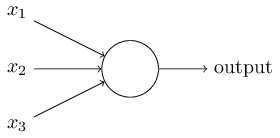
\includegraphics[width=\linewidth]{perceptron.png}
	\caption{A perceptron \cite{Nielsen2015}.} % to show under the picture
	\label{img:model} % to reference to the figure later
\end{figure}
In the figure \ref{img:model} the perceptron has three inputs: $x_1, x_2, x_3$.
To produce an output the perceptron posses of \emph{weights}: $w_1, w_2, w_3$ which represents
connection between input and output. Weights determine how important is an input to the output.
That said, the perceptron output is determined by whether the weighted sum $\sum_j w_j x_j$ is more or less
than some \emph{threshold} value:
\begin{equation} \label{perc:out}
	output = \begin{cases} 0, & \mbox{if } \sum_j w_j x_j \leq threshold \\ 1, & \mbox{if } \sum_j w_j x_j > threshold \end{cases}
\end{equation}

In shortly, this is a computational model which make a decision by weighting up
the evidence(input data) \cite{rosenblatt1962principles}.

Of course such a model is not capable of making complicated decisions, but
by extending the model to more complex network of perceptrons, we might improve the model.

\begin{figure}[H]
	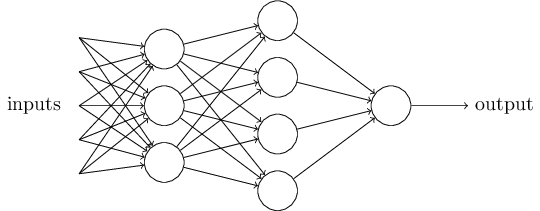
\includegraphics[width=\linewidth]{layer_perc.png}
	\caption{Two layer perceptron network\cite{Nielsen2015}.} % to show under the picture
	\label{img:layer_perc} % to reference to the figure later
\end{figure}

In the network shown on figure \ref{img:layer_perc}, we can observe
two layer of perceptrons. First layer will correspond to the first column of perceptrons
and will be responsible for the weighting up input, in contrast to second layer
(second column of perceptrons) which determines output by weighting up the result from
the first layer. Therefore second layer is located on more abstract level from input data
compared and can make more complicated decisions. Further layers might be capable
of making even more sophisticated decisions.

\subparagraph{Neural Network} Now that we know the way perceptrons work,
it's fairly easy to understand Neural Network. However we need to change
the mathematical notation a bit. For the sake of convenience, let's move
$threshold$ in equation \ref{perc:out} to the left part and replace it
with a variable known as the \epmh{bias} : $ b = -threshold$. Let's also simplify
the sum sign: $\sum_j w_j x_j$ by writing weights and input as vectors and use a dot product
to multiply them:
$\sum_j w_j x_j = W \cdot x$. Using changes described above we can rewrite the
equation \ref{perc:out} as following:

\begin{equation} \label{perc:with_bias}
	output = \begin{cases} 0, & \mbox{if } w \cdot x + b\leq 0 \\ 1, & \mbox{if } w \cdot x + b > 0 \end{cases}
\end{equation}

\emph{Bias} is a measure of how influential is a certain neuron on making output 1.
Some people also use more biological terms: the bias is a measure of how easy it is
to get an neuron to fire. To devise the neural network
next improvement over the perceptron network is that network should not be limited
to have an input only binary value, but any value. The same applies on the output.
Output being only binary value will limit the ability to make sophisticated decision.
Therefore we introduce a function known as \emph{an activation function} before
actually outputting a value: $output = g( W \cdot x + b)$ \cite{Nielsen2015} .

\subparagraph{Activation function} $g(\cdot)$ is known as an activation function.
Activation function helps to control the output and non-linearity of the network.
Activation function also plays a crucial role in multi layer architecture, where it helps
to prevent the values of each layer from blowing up.
For example, let's take a look at logistic sigmoid activation function which has
following form:
\begin{equation} \label{sigmoid_function}
	\sigma(z) = \frac{1}{1 + e^{-z}}
\end{equation}

TODO: write about tahn activation function

The use of the sigmoid activation will make a network to produce output to be
interpreted as posterior probabilities. Probability interpretation helps to provide
more powerful and more useful results \cite{Bishop1995}. There are a good variety
of activation functions but in this work we mainly will use the sigmoid activation function
and \emph{rectified function}. Rectified function is fairly simple.
It produces $0$ when input is less than $0$, and it does not change input value if
input is more than 0:
\begin{equation} \label{rect_function}
	R(z) = max(0, z)
\end{equation}
Now that we derived a concept of Neural Network, we can talk more about
what is called feedforward neural network and the terms related to it.
\paragraph{Feedforward neural network} is a network where the output
from one layer is used as input to the next layer. In feedforward NN
information is always fed forward in contrast to recurrent neural network(RNN)
where information can go in a loop. We will take a closer look at RNN in section
\ref{Recurrent Neural Network}.

\begin{figure}[H]
	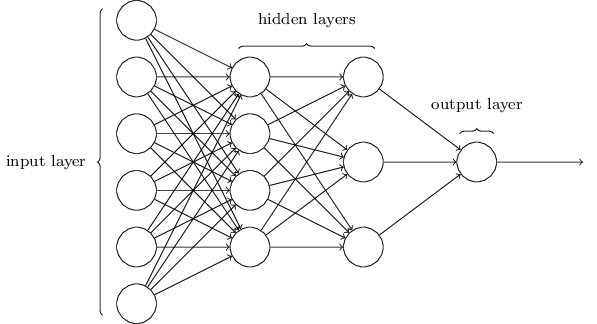
\includegraphics[width=\linewidth]{mult_layer.png}
	\caption{The architecture of neural networks\cite{Nielsen2015}.} % to show under the picture
	\label{img:mult_layer} % to reference to the figure later
\end{figure}

Basically Feedforward neural network is exactly
what we described above. Let's name different parts of feedforward NN:

\begin{itemize}
	\item Input layer - the leftmost layer in the network. The Neurons within
		input layer, called input neurons.
	\item Output layer - the rightmost layer in the network. The Neurons within
		input layer, called output neurons.
	\item Hidden layers - all the layers excluding input and output layers.
\end{itemize}

For example, the Neural network in figure \ref{img:mult_layer} consist of

\begin{itemize}
	\item 6 input neurons
	\item 2 hidden layers
		\begin{itemize}
			\item first hidden layer consist of 4 neurons
			\item second hidden layer consist of 3 neurons
		\end{itemize}
	\item output layer consist of one single neuron
\end{itemize}


\paragraph{Training}
As mentioned above Neural Network is capable of solving complicated
pattern recognition problems. However designing an neural network is not sufficient
for this. It's also requiring to train an network. In this paragraph we will
introduce learning procedure. But before going into learning, let's recap
how our neural network model looks like:

\begin{equation} \label{eq:nn}
	y = g(W * x + b)
\end{equation}
Where $g$ is an activation function, $W$ - weights, $b$-biases, $x$ - input data.
The space of different weights and biases values building a space of solution for
cetrain problem. The goal of the training is to find the best parameters
for neural network ($W, b$), that suited our problem.

\subparagraph{Training data} To solve pattern recognition problem we need to provide
a continuous feedback to NN, which NN can use to learn from. This feedback
in machine learning called \emph{training data}.
Training data consist of the input data samples
and appropriated outputs. You can think of training data as of an list of tuples:
${(x^{(1)}, y^{(1)}), (x^{(2)}, y^{(2)}), ..., (x^{(n)}, y^{(n)})}$ where $x$ - input,
$y$ - output (also known as ground truth), $n$ - amount of training examples. Neural network trained on training data
should be able to generalise the output on unseen input data.
The goal of the learning is to train network on training data and make it to capable of generalizing the output on unseen input data.

\subparagraph{Cost} In order to teach the model, it's essential to understand
what does it mean for an neural network to be good or to be bad. For this purpose
it's required first to define a \epmh{cost function}. Cost(also knows as error) is the metric
for the NN(or any other function approximation method), which represents how far of
the model is from desired outcome. If cost is big , our network does not work well.
With the cost function, it's possible
to define our training goal more precisely: the smaller our cost, the better our
model works, therefore the goal of the learning is to minimize the cost of our model.

\subparagraph{Types of cost} There are a plenty of ways to define cost of the model.
Let's consider the common type of cost function called \emph{mean squared error function}.
Mean squared error function has following form:
\begin{equation} \label{eq:mse}
	I_{W^\prime} = 1/2 * n * \sum_{i=1}^n (y_{W^\prime}(x^{(i)} - y^{(i)}) )^2
\end{equation}
\begin{itemize}
	\item $y_{W^\prime}$ - is our neural network function with the parameters ($W^\prime, b^\prime$),
	\item $x^{(i)}, y^{(i)}$ - is input and output of a training sample respectively.
\end{itemize}}

Another common type of function to measure the cost of NN known as \emph{cross entropy}.
In short, cross entropy gives a way to express how different two distributions are:
\begin{equation} \label{eq:cross_entr}
	I_{W^\prime} = - \sum_{i=1}^n  y_{W^\prime}(x^{(i)}) log(y^{(i)})
\end{equation}
where:
\begin{itemize}
	\item $y_{W^\prime}$ - is our neural network function with the parameters ($W^\prime, b^\prime$),
	\item $x^{(i)}, y^{(i)}$ - is input and output of a training sample respectively.
\end{itemize}}
\ref{Nielsen2015}


\subparagraph{Gradient Descent} \label{par:grad_desc}Once we defined our cost function, we need to find
a set of parameters $W, b$ which make the cost as small as possible. The most common
algorithm used to minimize the cost function called \emph{gradient descent}.
Let's explain the algorithm on an example function: $f = f(V)$,
where $V = \vec{v_1}, \vec{v_2},...$ are variables that we want to minimize.
Gradient descent uses partial derivative
to iteratively update parameters. Derivative of a function shows how function output
will change with respect to very, very small change in input $\Delta V $.
For example, partial derivative with respect to variable $\Delta{\vec{v_1}}$ will tell us, how different
the output will be $\Delta f $ if we change $\vec{v_1}$ on the small amount.
This property of derivative is used in gradient descent algorithm.
Essentially, the gradient descent
performs updates on the variables to be minimized according to partial derivative of the
cost function with respect to this variables. \\
Gradient descent adopt the following procedure.
Beginning with an initial guess for value $v= \vec{v_1}, \vec{v_2} ...$, we update the vector $v$
by moving a small distance in v-space in direction in which our function $f$ raises
most rapidly, i.e. in the direction of $- \Delta_V * f $. Iterating this process,
we can devise the new set of parameters $V^{(new)}$:

\begin{equation} \label{eq:gd_update}
	\vec{v_i^{new}} = \vec{v_i} - \alpha \frac{df(\vec{v_i})}{d\vec{v_i}}
\end{equation}
where $\alpha$ - is a small positive number knows as \emph{learning rate}.
Learning rate determines the smoothness of updates and it's very important to choose
it appropriately since if learning rate is too small the learning can be too slow, while, if
learning rate is too big, algorithm updates can be too big to achieve the minimum
(it can overstep the minimum).

Depends on the conditions this will converge to the parameters $V$ where the function
$f$ is minimized.
% Let's now substitute our loss function into gradient descent algorithm
One important things to notice is that, we can use the gradient descent algorithm only
if $f$ is differentiable. \cite{Bishop1995}

\subparagraph{Mini-batch Gradient Descent} Normally gradient descent algorithm
is associated with the update on the loss computed with whole set of training data,
while, gradient descent where updates is performed only using loss computed
on a small batch of data knows as \emph{mini-batch gradient descent}.
Much faster convergence can be achieved in practice using mini-batch gradient descent.
\cite{KarpathyAndrej2016}


% In large-scale applications (such as the ILSVRC challenge), the training data
% can have on order of millions of examples. Hence, it seems wasteful to compute
% the full loss function over the entire training set in order to perform only a
% single parameter update. A very common approach to addressing this challenge
% is to compute the gradient over batches of the training data.




% In other words, we want to find a set of weights and biases which make the cost
%  as small as possible. We'll do that using an algorithm known as gradient descent.


% We'll consider only two types
% training data
% cost function





\subparagraph{Backpropagation} In order to compute gradients in gradient descent algorithm
backpropagation algorithm is normally used. Backpropagation is the procedure of computing
gradients applying a gradient chain rules and updating the weights accordingly.
It performs first an forward update to receive the network's error value. This error
value then is back propagated beginning from output layer(neuron) through all neurons
till the input in order to associate it with extent of this error($\Delta$)
which an certain neuron is responsible
for. Once this extent is calculated, it performs weights update \cite{Rumelhart1986}.


\section{Recurrent Neural Network}

\paragraph{Why recurrent NN?} Motivation for recurrent neural network(RNN) is that
in contrast to feedforward neural network, RNNs are capable of having internal memory,
i.e. capable of memorizing information, therefore deal better with sequential input data.
RNNs are closer to the way human's brain works. We don't start our thinking scratch,
all of us have different background, memories and experience and based on this
we're making our own decision and actions. \\
As already mentioned in \autoref{chap:intro}, in this work
the network should be able attend to different locations within an image, i.e.
choose a location and process only area with respect to this location. The network then
incrementally combines the information from different location and based
on the knowledge(memory) extracted from a location, network chooses a new location to
attend. As you might notice since more steps need to be required, we will have sequential
data. Hence, RNNs are underlying concept for this work.

\paragraph{What is RNN} RNN is a special type of neural network architecture, which can
accept a sequence with an arbitrary length without changing weights of a network.
% Essentially, they are network who is capable of
RNN are capable of persisting the information by means of recurrences, i.e. including
the output of the network into next computational steps and summarizing this information
into an object called \emph{state}.
 \cite{Kriesel2007NeuralNetworks}.
\\
To simplify the understanding you can imagine RNN as an composition of identical
feedforward network, one for each step in time, passing the message to a successor.
Essentially, it's a computational unit that is repeated over and over again and
can be also thought as an for-loop.
One neural network in this composition known as \emph{RNN cell}.

\begin{figure}[H]
	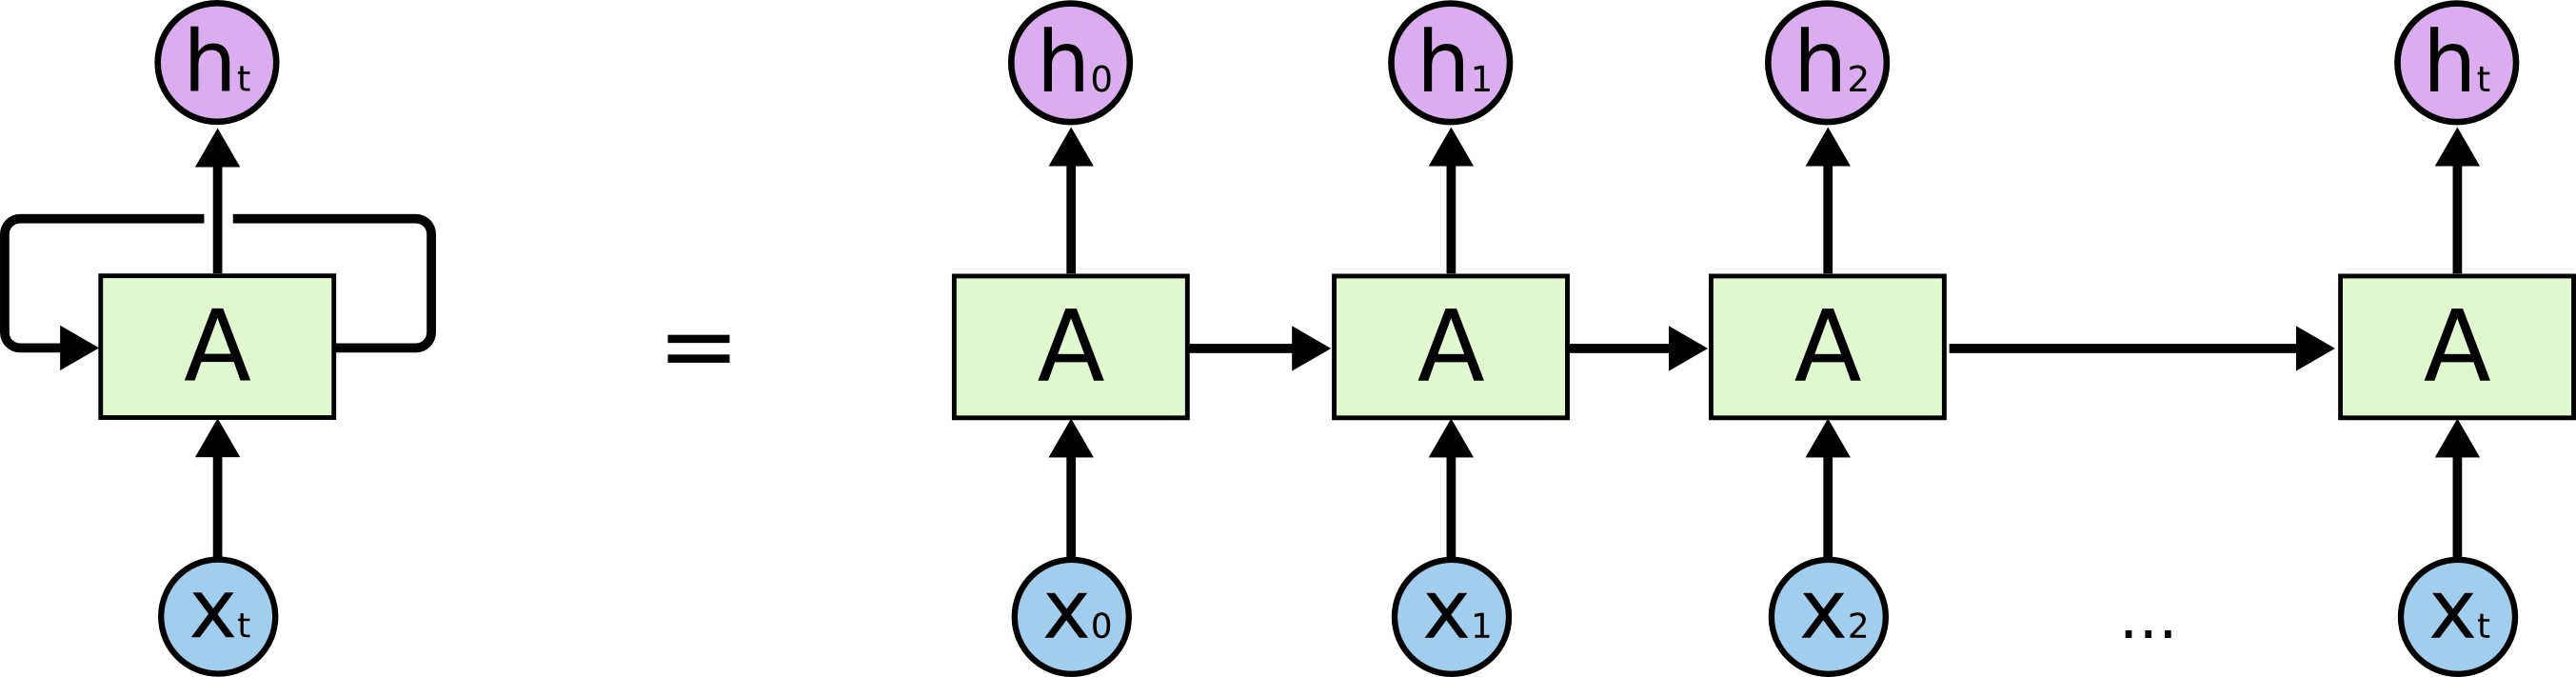
\includegraphics[width=\linewidth]{RNN-unrolled.png}
	\caption{Unrolling recurrent neural network(source: \cite{ColahChristopher2015})}
	\label{img:rnn_unrolled}
\end{figure}

On the right side of the figure \ref{img:rnn_unrolled} you can see an
unrolled RNN that accepts as input $x_0, x_1, x_2, ..., x_t$ and produces following
output: $h_1, h_2, ..., h_t$. One time step represents a layer in terms
of forward neural network.
The whole concept can be explained in the following
equation:

\begin{equation} \label{eq:rnn_basic}
	\begin{pmatrix}
		s_t \\
		o_t
	\end{pmatrix} = f
	\begin{pmatrix}
		s_{t-1} \\
		x_t
	\end{pmatrix}
\end{equation}
where:
\begin{itemize}
	\item $s_t, s_{t-1}$ - are states at time step $t$ and $t-1$ respectively,
	\item $o_t$ - is the output at time step $t$,
	\item $x_t$ - is the input at time step $t$,
	\item $f$ - is a recurrent function(normally called as RNN cell).
\end{itemize}}

As you might notice, the all calculations responsible for extracting and
memorising information performed in $f$, which provide knowledge about
specific \emph{RNN architecture(RNN cell)}.
Thus the choice of recurrent function $f$(RNN cell)
is essential for RNNs to work and remember information. There are a lot of variations
of RNN cells, but we mostly will consider one of the recent and
most widely known architecture called \emph{Long Short-Term Memory (LSTM)}.


\subsection{Long Short-Term Memory (LSTM)}
The reason that the vanilla RNN(Elman RNN cell \cite{Elman1990}) is not considered here,
because they are not able
to learn long term dependencies due to vanishing and exploding gradient problem \cite{Hochreiter1991}.
\paragraph{Long Short Term Memory networks(LSTMs)} are a special architecture of RNN cell,
capable of learning long-term dependencies. \cite{Hochreiter:1997:LSM:1246443.1246450}
LSTMs have the ability to remember new information and forgetting old, unnecessary information
using concept of gates. LSTM cell holds information in the object called \emph{state($C_t$)}
and only the gates are permitted to manipulate and change this state.
% These gates are responsible for the data in \emph{state}.
Gates are represented as an sigmoid layer and pointwise operation and will be explained
below.

\begin{figure}[H]
	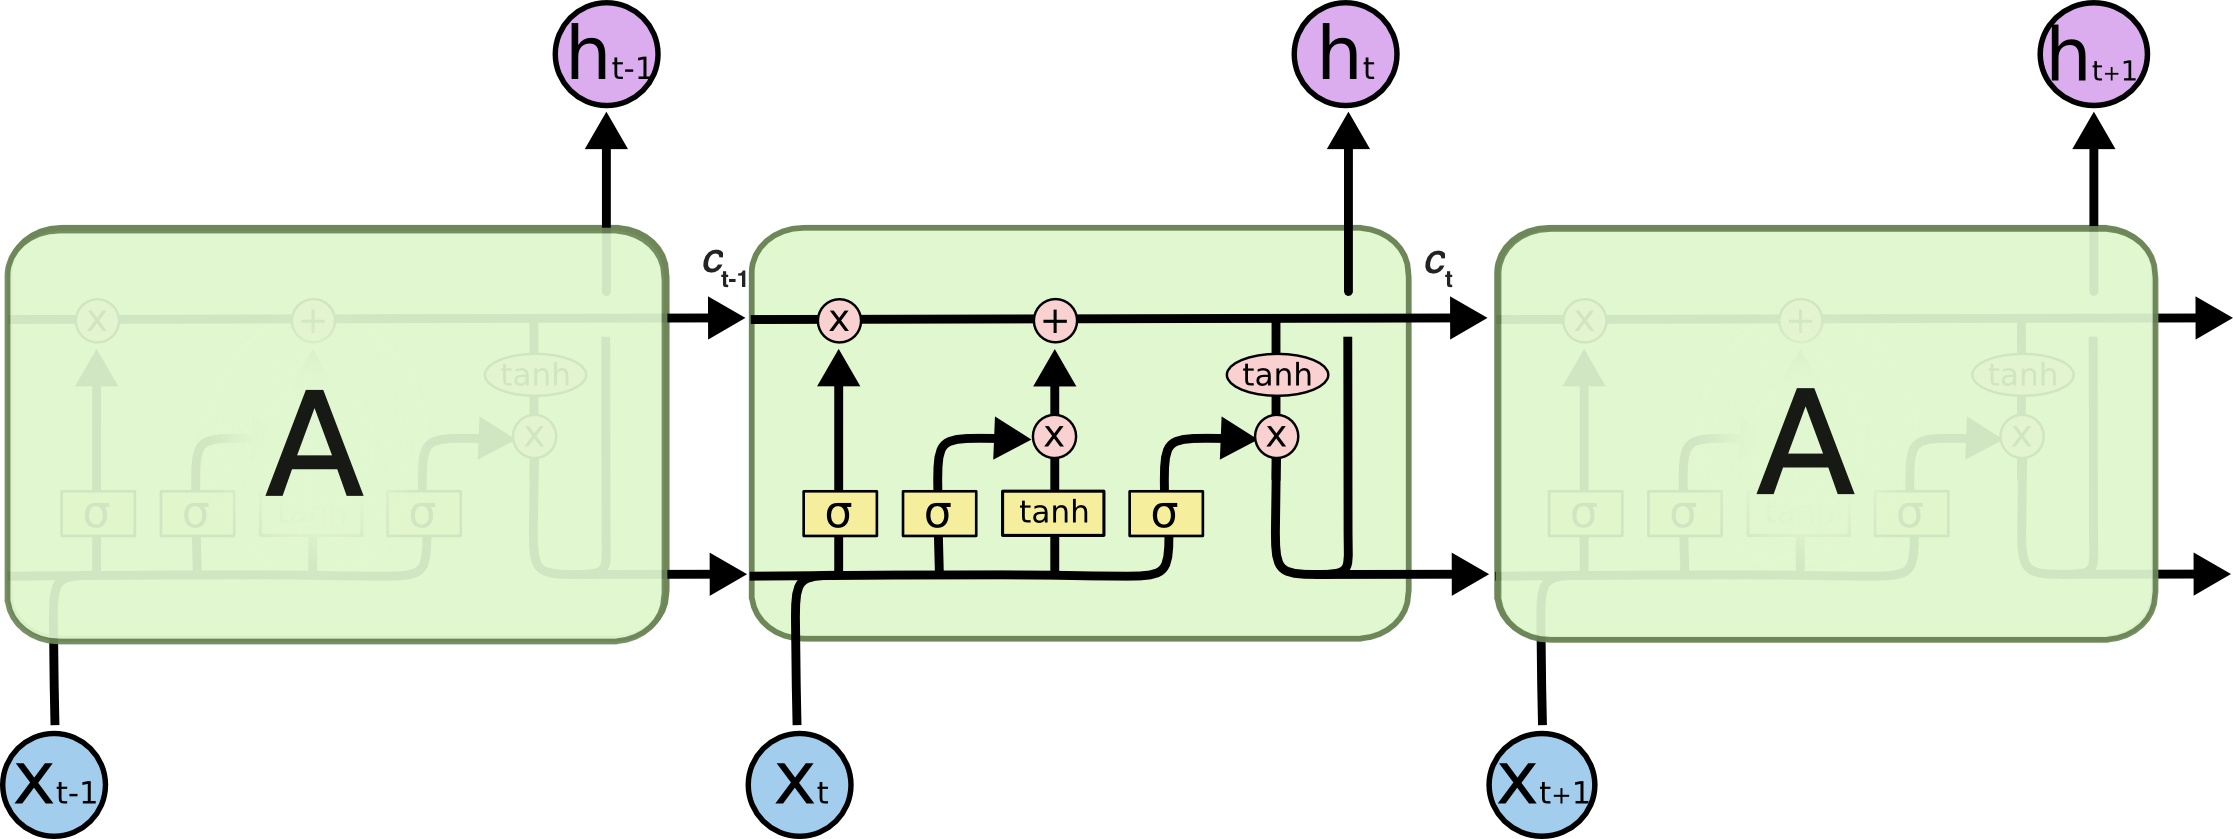
\includegraphics[width=\linewidth]{LSTM_inside.png}
	\caption{
		Structure of LSTM cell(Source: \cite{ColahChristopher2015}) \\
		An yellow square with $\sigma$ inside represents a neural
		network with sigmoid activation function, while yellow square with $tahn$ inside represents
		a neural network with tahn activation function.
		}
	\label{img:lstm} % to reference to the figure later
\end{figure}


As you can see from the figure \ref{img:lstm}, LSTM cell has four layers,
which build up three gates to interact with the state:
\emph{Forget gate}, \emph{Input gate}, \emph{Output gate}.

% Let's take a close look at key idea behind, this three LSTM gates:

\subparagraph{Forget gate layer}
The sigmoid layer that you can see on the right side is
called "forget gate layer". As you might notice from the name, this gate is responsible
for remembering information(or forgetting). It concatenates output from previous state: $h_{t-1}$
with the input at the timestep $t$: $x_t$. Then the result is fed to the neural network
with sigmoid activation function which produces an output with values from $0$ to $1$.
Where 0 means to completely forget the information and $1$ means to leave
the information in the state:

\begin{equation} \label{eq:forget_gate}
	f_t = \sigma (W_f \cdot [h_{t-1}, x_t] + b_f)
\end{equation}

\subparagraph{Input gate layer} composed of two networks: networks with sigmoid
and tahn activation functions. The first sigmoid network decides which values needed
to be updated and till what extent, while the network with tahn activation function create a
new candidate state value. Then the outputs from then networks are multiplied with each other
to create an update for the LSTM cell's state:

\begin{align} \label{eq:input_gate}
	i_t = \sigma (W_i \cdot [h_{t-1}, x_t] + b_i) \nonumber\\
	C_t^{(candidate)} = tahn(W_C \cdot [h_{t-1}, x_t] + b_C)
\end{align}

\subparagraph{Updating the state}
It's fairly simple now to update the old state $C_{t-1}$ using $f_t$ from equation
\ref{eq:forget_gate} to forget information and using new state candidate values
$C_t^{(candidate)}$ and it's extent $i_t$ from equation \ref{eq:input_gate}:

\begin{equation} \label{eq:update_state}
	C_t = f_t * C_{t-1} + i_t * C_t^{(candidate)}
\end{equation}

\subparagraph{Output gate layer} is responsible for the cell's output $h_t$.
This layer is allowed to read information from the state $C_t$ and decides what information
should be outputted.
\begin{figure}[H]
	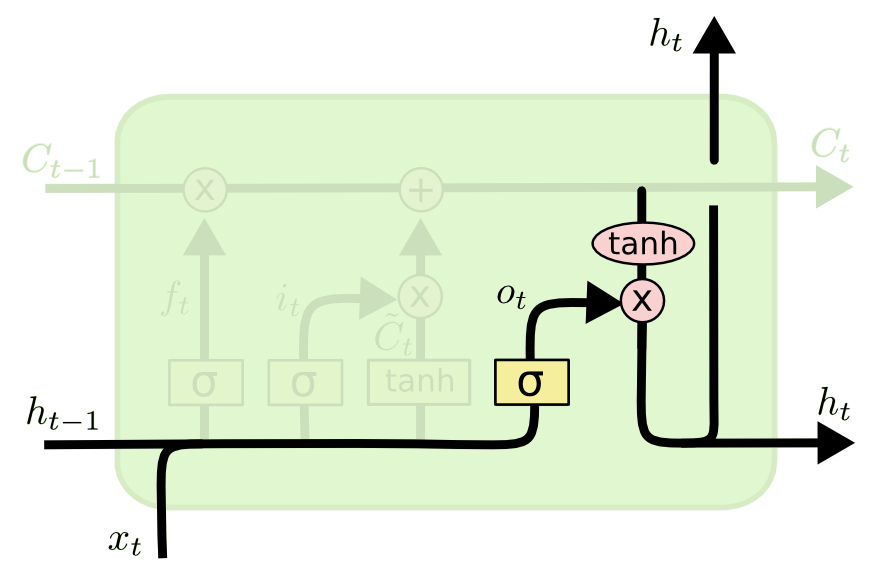
\includegraphics[width=\linewidth,height=6cm,keepaspectratio]{LSTM_out.png}
	\caption{
		LSTM's output gate layer (Source: \cite{ColahChristopher2015})
		}
	\label{img:lstm_out}
\end{figure}

As you can see from figure \ref{img:lstm_out}: firstly, state cell goes
through tahn function and then multiplied
with output from the neural network of output gate layer:

\begin{align} \label{eq:out_gate}
	o_t = \sigma (W_o \cdot [h_{t-1}, x_t] + b_o) \\
	h_t = o_t * tahn(C_t)
\end{align}

$h_t$ is the output of LSTM cell at time step $t$ as well as the input
for RNN cell at time step $t+1$. The gates stabilize the state and solve the
vanishing gradient problem, hence it's very important for an LSTM
cell to work.\cite{Goodfellow-et-al-2016}

% TODO: just follow the stuff from colah's blog.
% * Talk about the gates
% * explain all three gates in particular
% * write equations
% * write shortly about backpropagation through the time.
\paragraph{Backpropagation Through Time} Taking into account that RNN nets
share all weight between layers(time steps), there is a specific
technic for computing
gradient when training the network called \emph{Backpropagation Through Time(BPTT)}.
It propagates the error all the way back through the time to the time step 0,
that's the reason it's called BPTT. \cite{werbos:bptt}
% hence why it's called
% hence is the name.

We can think about it as using feedforward neural network's backpropagation
but with the constrain that the weights of the layers should be the same.
However as RNN might have a hundred of thousands time steps it is common
practice to truncate the backpropagation only back to few time steps, instead
of backpropagating it to the first time step.





\section{Reinforcement Learning}
\subparagraph{Why reinforcement learning?}
As you might recall from \autoref{chap:intro}, the recurrent visual attention model
extracting information from a picture by attending to certain locations of the picture
and aggregating the information from these locations. This property will make our network
avoid locations with insignificant information, hence ignore clutter. In order to teach the network
output next location to attend given previous location, we need to provide training data to
the neural network. The problem is here, that we don't know the right answer for this.
We can only say whether the network made a right classification decision after the network
has already chosen several locations. Consequently, the training of the network parameters will
be a very difficult task. As previously mentioned in \autoref{par:grad_desc}, using gradient descent
with backpropagation for training NN is possible only with differentiable cost function like
mean squared error function or cross entropy function. However, we can't use this functions without
the knowing the right answer, therefore defining the cost function would be a complicated task.
This sort of tasks is studied by a field of machine learning called \emph{reinforcement
learning(RL)}. Reinforcement learning concerned with teaching an agent to take actions based on
reward signal, even if this signal is delayed. These agents are trained to maximise the total
sum of such reward signals.

% \subsection{}


% used the idea
% need to decide next location based on the predecessor location \
% why do we need it our work?


\paragraph{The Basics and main components}

MOMDP
Reinforce rule
reducing variance by using advantage function

% Generally, recurrent networks are net- works that are capable of influencing themselves
% by means of recurrences, e.g. by including the network output in the following
% computation steps. There are many types of recurrent networks of nearly arbitrary
% form, and nearly all of them are referred to as recurrent neural networks.
% As a result, for the few paradigms introduced here I use the name recurrent
% multilayer perceptrons.
% Apparently,
%  to provide the new location to attend based
%
%
% The model is a recurrent neural network (RNN) which processes inputs sequentially,
% attending to different locations within the images (or video frames) one at a time,
% and incrementally combines information from these fixations to build up a dynamic
% internal representation of the scene or environment. Instead of processing an entire
% image or even bounding box at once, at each step, the model selects the next location
% to attend to based on past information and the demands of the task.





% Each of those perceptrons is making a decision by weighing up the results from the first layer of decision-making. In this way a perceptron in the second layer can make a decision at a more complex and more abstract level than perceptrons in the first layer
% In this network, the first column of perceptrons - what we'll call the first layer of perceptrons - is making three very simple decisions, by weighing the input evidence. What about the perceptrons in the second layer?
% . And even more complex decisions can be made by the perceptron in the third layer. In this way, a many-layer network of perceptrons can engage in sophisticated decision making.

% To make it clear here is a vocabulary that will be used throughout the paper:






% f(n) = \begin{cases} n/2, & \mbox{if } n\mbox{ is even} \\ 3n+1, & \mbox{if } n\mbox{ is odd} \end{cases}




% The problem that we trying to solve in this paper is known as
% pattern recognition problem. We trying to recognize pattern in images
% in order. The problem can be described
% as searching for patterns in data like image, text, sound and etc. An example
% of the problem can be to find a tree in a picture.

% What is special about? desribe few properties of neural network
% differencet between Conventional algoritms
% what else is usable for




% \subparagraph{} What is meant here by computation.
% \subparagraph{Perceptron}


% biases weights
% - shortly how it works, a simple example but clear example. Better about MNIST data.
% ona layer network
% multi layer network
%
% \paragraph{Basic concept of neural network}
% There are a good variety of
% explain the example in terms of the elements
% layers, activation function. How output is produce.
%
% - about learning weights/ parameters , about data. Ground truth.
%
% - write shortly about how one updates parameters. About stoschastic gradient descent
%
% - different activation functions
% - learning rate
% - a little bit about backpropagation.

    \chapter{Analysis}
\label{ch:analysis}
The main objective of this work will be to build an extensible prototype,
which will be built on the model of visual attention and additionally
extended to classify
a set of images. This chapter discusses the main concerns
that have to be taken into consideration in order to achieve the objective.

Firstly, let's define the clear problem statement:

\textit{
	Given a dataset where each sample consist of a group of images.
	A certain label is asserted to every sample in a dataset. The goal is
	to build a extensible prototype upon RAM that is capable of classifying
	this samples. The prototype is the resemblance of the RAM model with
	with ability to accept the above mentioned dataset.
}

\\

% TODO:
% * name the section regarding the quality
% * finish the Analysis chapter:
% ** what is best practices in python?
% ** what is best practices in general?
% ** Limitations of the preivous work> fullfil the lsit belowe

\section{Quality concerns}
\label{sec:quality_concerns}
This statement make it clear that prototype should be extensible. Extensible
means that other people(including author itself) are able to extend the
prototype. People should comprehend the code as well as start and configure
procedures in order to extend the prototype. Therefore following best practices
and conventions, using widely known frameworks, producing clean and readable code
to stay consistent with other modern software is an important
point of this work.

It's more convenient to talk about conventions once programming language and
libraries are chosen for this work.
\paragraph{TensorFlow}

There is a big variety of frameworks and libraries used in machine learning.
Among the famous libraries is library called TensorFlow. TensorFlow is an open
source library developed and maintained by engineers from Google \cite{tensorflow2015-whitepaper}.


TensorFlow framework has gained a huge popularity among machine learning
community as well as in industry compared to another framework \cite{DBLP:journals/corr/Goldsborough16}.
TensorFlow is an open source software library that makes computations more
efficient by building a computation graph and deploying them to one or more
CPUs or GPUs.


TensorFlow framework gives a wide variety of statistical distributions, wide
range of loss functions, and a huge amount of neural network algorithms while
not necessarily losing  flexibility. In order to make learning process traceable,
TensorFlow provides TensorBoard, which is a web interface for graph visualization
built directly into TensorFlow.
TensorBoard is an important and uniq feature that excels TensorFlow from similar
libraries; it dramatically improves debugging experience as well as helps
for understanding models developed using TensorFlow.
Aforementioned features of the framework as well
as it's great API for Python is a great fit for this work.

The current work will use Python as programming language, as it's one of
the most popular language among machine learning community.


\paragraph{Code conventions}
Now that we assigned interfaces, let's define conventions that this work
will follow. As TensorFlow recommends using PEP 8 style guide to stay consistent
with community \cite{TfWeb}. PEP 8 gives the set of rules about how to lay out
the code, how to name functions, methods and classes and others code style related
aspects \cite{Rossum}. PEP 8 linter is also integrated in the project, which checks the code
automatically on presence errors against PEP 8 style guide,
therefore simplifies the development workflow.

PEP 257 convention is also considered as this will help to avoid errors when
generating documentation. PEP 257 convention set rule about organizing
docstrings in Python \cite{Goodger2001}.
Overall, the work follows The Hitchhiker's Guide to Python, which advises
about the way of testing, organizing and documenting the code \cite{Reitz}.

\paragraph{Code patterns}

Despite that a lot of code from researches are not following and not using code
pattern, it's really simplifies understanding and reasoning about the code, especially
while extending or adjusting the model. Therefore using code patterns
is highly recommended. We will introduce the code patterns, which
is recommended in the functional programming from \cite{beck1997smalltalk},
because python supports the concept of functional programming.
To follow are also general well-known code patterns that are taken from
\cite{martin2003agile}, \cite{Eckel2017}, \cite{Gamma:1995:DPE:186897}.
Below is a list of this code pattern recommendations:

% design patterns
\begin{itemize}
	% done
	\item Composed method - it's saying that methods should
		have one identifiable task. Additionally to this, all operations
		performed in the function should be on the same level abstraction.
		This will increase flexibility of the methods and prevent
		from confusing code and mistakes. \cite{beck1997smalltalk}
	% done
	\item Extract method - when one method is too long, one should try to
		extract some part of it into another function taking into account that this
		function should be useful on its own. \cite{1999:RID:311424}
	% implement or throw it away
	\item Method object -  normally applied when one can't use extract method
	 	on a function because new function would take a lot of parameters
		from the original method.
		The idea is to create a small class that will hold this parameters
		as properties and then to create small methods within this class without
		passing the parameters to it but instead access them as class properties.
		\cite{beck1997smalltalk}
	% implement
	\item Method comment - instead of having a comment close to not
		self-explanatory statement, one should rather create a function
		with self-explanatory name that holds this statement.
		Most comments are redundant, therefore one can simplify
		the system by introducing small methods.
		\cite{beck1997smalltalk}
	% done
	\item Temporary variable - instead of having very long expression, it's recommended
		to assign part of the expression to a variable. This variable can also have
		the self-explanatory name, consequently increasing the readability of the code.\cite{beck1997smalltalk}

	\item Simple Enumeration Parameter - having a simple name of a parameter
		when iterating over enumeration: \lstinline{for each in plugins:} \cite{beck1997smalltalk}
	% done below
	\item Cascade pattern - when a method of a class doesn't return any value,
		one can return instance of the class in order to be able to call a
		next method of the instance in cascade way: \lstinline{self.doThis().doThat()}.\cite{beck1997smalltalk}
	% done below
	\item Single responsibility principle - it forces every class to have only one
		clearly distinguishable responsibility.\cite{martin2003agile}
	% done
	\item Duck Typing - is a specifically to python, a design principle that
		says that if an object has a certain desired functionality it doesn't not matter
		what of nature the object is.
	% % bullshit
	% \item Composition over inheritance - it's design pattern which obligates
	%  	to use composition rather than inheritance. \cite{Gamma:1995:DPE:186897}
	% done
	\item Iterator - is a design pattern that says to access values of a list
	 	without exposing the list \cite{Gamma:1995:DPE:186897}. It's built into python language itself and
		can be used with syntax like \lstinline{for .. in ..} or \lstinline{next()}.
	% done
	\item Singleton - design pattern that obligates a class to be
		instantiated only once. \cite{Eckel2017}
\end{itemize}

% keep a system decoupled and thus easier to refactor, change, and redeploy
% https://en.wikipedia.org/wiki/Separation_of_concerns
% https://refactoring.com/catalog/replaceMethodWithMethodObject.html
% https://refactoring.com/catalog/extractMethod.html
% http://codebetter.com/jeremymiller/2006/12/03/composed-method-pattern/
% inderact variable acces
Since ML programming is more method oriented, the most pattern above concentrated
on how to keep functions readable, precise and flexible. In this work we will follow
these patterns.

We will see examples of those patterns in the \autoref{ch:design}
and \autoref{ch:implementation}.

To recap, the prototype should be not only a good start for making further
improvements on large scale objects but also be a piece of software that bears the
following properties: extensible, well documented, integrable with other
softwares, easy configurable, readable code.


\section{Analysis of the previous work}
As we will build the current model upon RAM described
in \autoref{sec:ram_model}, it makes sense to look over the existing implementations
of the RAM model.
The authors of RAM paper haven't provide the implementation, but
fortunately there are few implementations built by open source community.
It's common to see that people, who working on a model as open source project,
are often do that in their free time. As a consequence, it is expected that those model
are not high-quality prototypes, therefore in order to rely on the project
one needs to be meticulous while choosing one.
Following criteria were considering when choosing the model for the basis
of this work:

\begin{itemize}
	\item Structure and readability of the code - at least presence of the basic structure
	\item Configuration - it should be comprehensible how one can change parameters
		of the model
	\item Reproducible results
	\item Presence of basic documentation
	\item Framework - as we have already chosen TensorFlow, projects built upon
		TensorFlow are preferable.
\end{itemize}

After doing the research and taking into account the above listed criteria,
the choice fell on the project from github user 'zhongwen'. We will refer to
this implementation as \emph{
	basic RAM implementation
	\footnote{The original project is located on github: https://github.com/zhongwen/RAM .}
}.

This project is built using TensorFlow framework.

\subsection{Advantages over original RAM paper}
Building a machine learning software is not as straight forward as building
conventional software. In machine learning, in order to achieve high accuracy
one uses different methods which are normally hard to comprehend without knowing
the theory behind it. Absence of testing is one another point which makes it
harder to understand others code. Considering this circumstances careful
analyzing of the approaches used in the basic RAM implementation
is desired for the success of this work.

\paragraph{Inference} in the current work was performed differently from what was
described in \cite{DBLP:journals/corr/MnihHGK14}.
% The method used in \cite{DBLP:journals/corr/MnihHGK14} was to running
% $M$ episodes on the one sample following by updating the parameters of the network.
Let's take a look at how the gradient of objective function is calculated in \cite{DBLP:journals/corr/MnihHGK14}:
\begin{equation} \label{eq:}
	\Delta_{\theta} J = \frac{1}{M} \sum_{i=1}^M \sum_{t=1}^T
		\Delta_{\theta} \log \pi_{\theta}(u_t^i| s_{1:t}^i) (R_t^i - b_t)
\end{equation}
where $J$ - is a cost function, $M$ - number of episodes,
$T$ - is a time step where the agent is forced to make a classification decision,
$s_{1:t}^i$ - are state sequences obtained by
running the current agent $\pi_{\theta}$ for $i = 1 . . .M$ episodes,
$b_t$ - baseline to reduce variance, $u_t_i$ - action at time step $t$
of episode $t$.

As we can see the gradient is calculated based on running $M$ episodes.
Firstly, the agent chooses sequentially $n$ location and make a classification
decision. Then we run $M$ similar episodes like this. After this,
we compute the gradient. The basic RAM implementation used slightly different
approach. It does not run multiple episodes to update the parameters, but instead
it does update parameters on every episode. However it duplicates the same
samples $M$ times and then obtain $M$ different outputs and average them.
This practice was introduced in \cite{DBLP:journals/corr/BaMK14}.
It was also indicated that running attention model multiple times on each
image with the classification predictions being averaged gave the best
performance \cite{DBLP:journals/corr/BaMK14}.


\paragraph{Adam Opmitimizer} It also worth to notice that instead of stochastic
gradient descent that was used in RAM paper, the basic RAM implementation using Adam optimizer
from \cite{DBLP:journals/corr/KingmaB14} with exponentially decaying learning rate,
which theoretically should improve performance. \cite{DBLP:journals/corr/KingmaB14}


\paragraph{Gradient clipping} In contrast to RAM paper, the basic RAM implementation
additionally clipped the gradient values by global norm of their values to prevent the vanishing
and the exploding gradient problems \cite{Pascanu2012}.


\subsection{Limitations}
Unfortunately, the basic RAM implementation used old version of TensorFlow,
which was unstable at that moment, therefore migration of the project
to the latest TensorFlow version is required\footnote{
	Migration was performed according to TensorFlow migration
	guide: https://www.tensorflow.org/install/migration
}

Looking at basic RAM implementation purely from software engineering side,
one can observe severals flaws. Not following python conventions as well
as lack of design patterns and partial presence of incoherent structures in the code
are known obstacles when analyzing and extending the code.
Therefore code is required to be refactored and cleaned,
as well as restructured and documented under the conventions and
practices described in \autoref{sec:quality_concerns}.

% It's very common to see that researchers don't worry much about the
% building well-engineered prototype as most of them are not software engineers.
% Mostly the are big experts at math, it's understandable since excelling both
% fields is very time consuming. The basic RAM implementation is not an exception.
% The code is required to be refactored and cleaned, as well as restructured.

As of functional requirements, lack of one feature was detected in basic RAM implementation.
As you can remember from \autoref{sec:ram_model}, glimpse sensor is taking
multiple patches from an image, where each patch is taken at different resolution.
The basic RAM implementation is not capable of taking multiple patches,
but only a single one. Without ability of taking multiple patches within a glimpse,
accuracy of inference will more likely to decrease. Therefore this functionality
should be available in the work in order to achieve better results.

Additionally to this, TensorBoard wasn't configured in basic RAM implementation.
Training such massive model as RAM can be complex and sometimes confusing.
Tools like TensorBoard make models easier to understand, debug
and optimize, therefore having fully configured TensorBoard is another
prerequisite for a good prototype.




% TODO for tomorrow:
% * revise the paragraph above, be precise and careful and think about all problems/ DONE
% * limitations are important, also say that everything below is opinionated and / DONE
	% a this a pure look from software engineering side
% * write about probably about the importance of the design patterns()
% * finish the analysis




% Original project contained
% a lot of style errors and had many inconsistencies in the code with respect
% to code style.
% The code is not followed by conventions therefore one can notice

% tesnorflow version
% tensorboard
% structure
% was not suitable for taking multiple patches
% very start level of documentation
% Absence of basic documentation


% \paragraph{paragraph name}









% \paragraph{Analysis}



% Machine learning is a field where
% But before actually building the extension upon this project,
%
%
% can have lack of documentation and b
% This can be a reason for having
% due to lack of resources
% As the implmentations provided by open source community
% often have lack of documentation and
%
% One of them due to certain level of readability is more attractive for this work.
% While the project is way more readable compared to others, it's still in the need
% of refactoring.
% This code is implemented by using tensorflow framework.


\section{Extension}
\label{sec:extension}
In order to fulfill the objective of this work, it's required to extend the basic
RAM implementation in a following way: it should accept a group of images as input
and based on that input make a classification decision. Group in this case means
more than one image(e.g. 2,3 or 5 images). More formally:
\textit{given a group of images, extended model returns a probability distribution over
$K$ different outcomes, where $K$ - is amount of classes in the classification problem.}
We'll refer to amount of the image in a group as $n$.

This section will discuss several ways of how to achieve that.
In the figure \ref{fig:ram_model_arch} you can see original architecture of RAM.
The potential extension variations listed below will use the notation, which
was presented in \autoref{sec:ram_model}.

\begin{figure}[h!]
	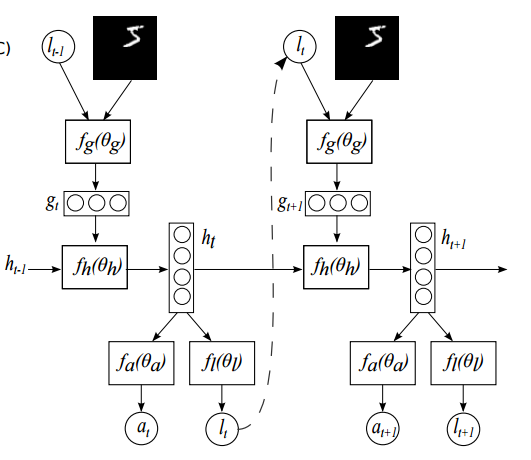
\includegraphics[width=\linewidth,scale=0.4]{ram_model_arch}
	\caption{Original architecture of RAMS(Source: \cite{DBLP:journals/corr/MnihHGK14}).}
	\label{fig:ram_model_arch}
\end{figure}

\subsection{Picker network}
\label{subs:picker_net}
You might remember the output of LSTM cell $h_t$ in \cite{DBLP:journals/corr/MnihHGK14}
which was described in \autoref{sec:ram_model}.
The external output is used
in the action network $f_a(\theta_a)$ as well as in location network $f_l(\theta_b)$
as shown in figure \ref{fig:ram_model_arch} to produce a classification decision or
next location respectively. In a similar way, we can invent a new network that takes as
input the LSTM cell's output $h_t$, have parameters $\theta_p$ and outputs
the probability distribution over $n$. We shall call this network
\emph{picker network}. The purpose of the picker network is to pick an image
in the group to explore appropriate image, hence the name. By manifesting
this extension, the model as a whole will have three neural networks consuming
the output of LSTM cell $h_t$:
\begin{itemize}
	\item Classification network $f_a(h_t; \theta_a)$ - makes a classification
		decision after $T$ number of time steps.
	\item Location network $f_l(h_t; \theta_l)$ - decides where to allocate the next glimpse
	on the picture.
	\item Picker network $f_p(h_t; \theta_p)$ - decides what picture to allocate the next glimpse on.
\end{itemize}

All of networks above have a similar structure:
\begin{align} \label{eq:picker_network}
	f_a(h_t; \theta_a) = Softmax(Linear_{\theta_a}(h_t)) \\
	f_l(h_t; \theta_l) = Linear_{\theta_l}(h_t) \\
	f_p(h_t; \theta_p) = Softmax(Linear_{\theta_p}(h_t))
\end{align}
where $Z$ - is a normalizing constant, $Softmax$ - is softmax activation function
$Linear_{\theta}(x)$ - represents
a linear transformation $Linear_{\theta}(x) = W_{\theta}x+b_{\theta}$ with weights
$W_{\theta}$ and bias $b_{\theta}$.


\subsection{Deep attention model}
\label{subs:deep_att_model}
This idea was inspired by the approach used in \cite{DBLP:journals/corr/BaMK14}.
Idea is to completely separate classification network from location network
by introducing new RNN layer on top of the current RNN layer.

\begin{figure}
	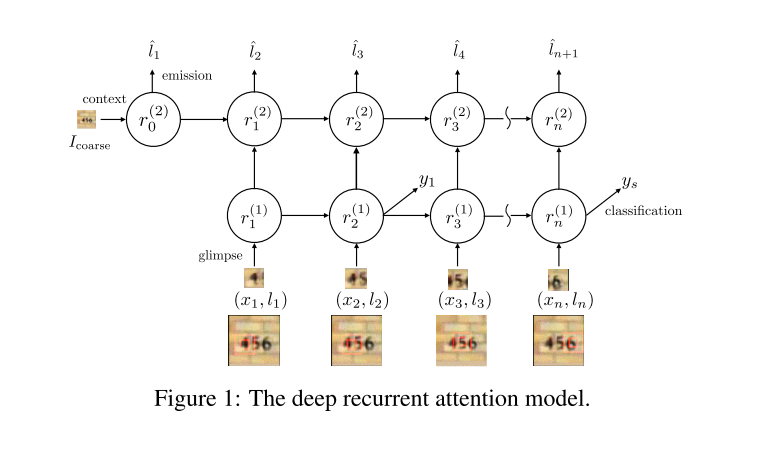
\includegraphics[width=\linewidth,scale=0.7]{deep_attention_model.png}
	\caption{Source: \cite{DBLP:journals/corr/BaMK14}}
	\label{fig:deep_att_model}
\end{figure}

In figure \ref{fig:deep_att_model} you can observe first RNN denoted $r^{(1)}$ which works
the same way as was described in \autoref{sec:ram_model}. Output of RNN $r^{(1)}$
was consumed by location network and classification network in \cite{DBLP:journals/corr/MnihHGK14}.
This will be different in current approach. We can describe it as following:
We introduce new RNN $r^{(2)}$ on top of first RNN:
\begin{itemize}
	\item The new RNN is initialized by output from convolution
		network(called Context Network) applied on the down
		sampled low-resolution version of input image.
		The feature vector outputted from convolutional layer
		provides sensible hints on where
		the potentially interesting regions are.
		The reason behind it was described in \cite{DBLP:journals/corr/BaMK14}:
		\blockquote{The existence of the contextual information(feature vector),
		however, provides a
		“short cut” solution such that it is much easier for the model to
		learn from contextual information than by combining information
		from different glimpses}
	\item The new RNN takes as input the output of RNN $r^{(1)}$:
		$r_n^{(2)} = f_{r^{(2)}}(r_n^{(1)}, r_{n-1}^{(2)})$,
		where $r_n^{(1)}$ - is the output of RNN $r^{(1)}$ at time step $n$,
		$f_{r^{(2)}}$ - is RNN cell function(e.g. LSTM cell),
		% $r_n^{(2)$ and $r_{n-1}^{(2)}$
		  $r_n^{(2)}$ and $r_{n-1}^{(2)}$ are outputs of RNN $r^{(2)}$
		  at time step $n$ and $n-1$ respectively.
	\item The output of new RNN is used to produce next location.
		The output is fed into fully connected network, which maps
		the feature vector produced by new RNN into coordinate object $[i, (x,y)]$,
		wherer $i$ - is a index in the group of images.
\end{itemize}

The reason for having the second RNN is to implicitly
represent decision about location and
prevent using location information in classification. Separation is crucial:
first RNN network is responsible for
classification, while second one for choosing the right location.
One state will hold information about classification, while the state of
RNN cell on the top will hold information about locations.
Advantage of this work is having this separation of concerns between
location and classification information which theoretically should improve the model.
This approach we will call \emph{Deep attention model}.

\subsection{Exploration network}
In original RAM paper, model is required to execute a number of
steps before making classification decision:
\blockquote{
The attention network used in the following classification experiments made
a classification decision only at the last timestep $t = N$.
}\cite{DBLP:journals/corr/MnihHGK14}
It was also suggested as a further improvement to introduce new action
which decides when model should stop taking further glimpses:
\blockquote{
Finally, our model can also be augmented with an additional action that decides
when it will stop taking glimpses. This could, for example, be used to learn a
cost-sensitive classifier by giving the agent a negative reward for each glimpse
it takes, forcing it to trade off making correct classifications with the cost of
taking more. \cite{DBLP:journals/corr/MnihHGK14}
}

We can use alter this suggestion by introducing a new action which
instead of indicating when the model should stop taking new glimpse, will
indicate when model should take a next image in a group. Once there is no more images
we can force the model to make a classification decision.

We introduce new network which take as input the state of RNN cell, and outputs
probability distribution over two actions which correspond to whether the model
will stop taking new glimpses
or continue to explore image.
We shall call this network \emph{the exploration network}.

By manifesting
this extension, similar to the approach described in \autoref{subs:picker_net},
the model will have three neural networks consuming
the output LSTM cell $h_t$:
\begin{itemize}
	\item Classification network $f_a(h_t; \theta_a)$ - makes a classification
		decision after $T$ number of time steps.
	\item Location network $f_l(h_t; \theta_l)$ - decides where to allocate the next glimpse
	on the picture.
	\item Exploration network $f_e(h_t; \theta_e)$ - decides whether the next glimpse
	should be taken
	from the $i$ image from the group or from the $i+1$ image.
\end{itemize}

New exploration network computes the distribution in the following way:
\begin{equation}
	f_e(h_t; \theta_e) = Softmax(Linear_{\theta_e}(h_t))
\end{equation}

The main advantage of this approach is the flexibility since it can easily be combined
with deep attention model introduced in \autoref{subs:deep_att_model}. This
approach can be also augmented with following actions:
\begin{itemize}
	\item First Action - go back, that is, take previous image from the group of images.
	\item Second Action - go forward, that is, take next image from the group of images.
	\item Third Action - finish, that is, stop taking glimpse and do the classification decision.
\end{itemize}

There is no theoretical to prove which one from the extensions will work better,
therefore testing them with experiments is required.
\section{Dataset}
\label{sec:analysis_dataset}

Before starting the construction of the model, one requires to think about an appropriate
dataset on which the model can be tested.
MNIST dataset\footnote{The MNIST data is hosted on \cite{LeCun2010}} is recognized
as being the simplest dataset among the computer vision
community, therefore building a dataset upon it would be easier. The simplicity of dataset
would help to understand problems occurring while developing a model.
Additionally to this, from researchers from google
Deepmind used MNIST to evaluate RAM, which indicated that MNIST data would
be good fit for the extension as well. \cite{DBLP:journals/corr/MnihHGK14}


\paragraph{MNIST Dataset} is dataset of scanned handwritten images, each labeled
from from set: $\mathcal{A} = \{0 .. 9\}$, where $\mathcal{A}$ - is a set of available
classes in MNSIT dataset. You can see an example of 4 digits in figure \ref{fig:mnist}.
Additionally, it includes label for each of the image.

\begin{figure}[h!]
	
\includegraphics[width=\linewidth,scale=0.4]{MNIST}
	\caption{MNIST example (Source: \cite{tensorFlowSite})}
	\label{fig:mnist}
\end{figure}

For example, in the figure \ref{fig:mnist} the labels are 5, 0, 4 and 1.
Each images consist of $28\times28$ pixels, therefore an MNIST image would
be an array of size $784$.

MNSIT dataset consist of 55,000 training samples, 10,000 test samples, 5,000 validation samples.
Requirement for the dataset can be formulated as following:\\
\textit{Each sample in the dataset should contain fixed number of images. Amount of images
in an sample should be more than 1. The dataset should have at least two classes,
which are used to label each of the sample. The dataset should provide enough
data to train, validate and evaluate the model.}



% There is different variations for building the dataset of group of images from MNIST dataset.
% One of them can be as simple as bringing two different numbers together and adding a
% noise image, which shouldn't have an influence on the outcome.
\subparagraph{Procedure}
We should come up with the dataset that will fulfill the requirements above.
One way of doing it could be described as following:
having limit of 10 classes in MNIST dataset, we decide about the class(or classes) of images
that hold information relevant for classification decision(it can be f.e. classes
labeled with 4 and with 3 in MNIST),
we'll refer to those images as non-noise images. Subset of classes of non-noise image
we denote as: $\mathcal{D} = \{d_1,..., d_n\}$.
We'll have also images which does not
contain any information relevant for decision making, we'll refer to this images
as noise images. Noise images is generated using images from classes that
are mutually exclusive with classes of non-noise images:
$\mathcal{T} = \mathcal{A} / \mathcal{D}$, where $\mathcal{T}$ - is a subset of classes $\mathcal{D}$
for labeling noise images: $\mathcal{T}\subset \mathcal{D}$.
% However, it's possible that $\not\subset$ TODO: finish it.
We then decide about the amount the images in a group $n$.
We then choose the number $k < n $ which is going to be amount of noise images
per sample in dataset.

% we choose one(or more) from this images(f.e. example image) and will call it(them) noise image(s) and refer
% to the amount of noise images as $k$.

We then divide the original MNIST dataset into two:
\begin{itemize}
	\item First dataset - consisting of noise images, where each sample is a group(array)
		of noise images with the size of $k$.
	\item Second dataset - consisting of non-noise images, where each sample is a group(array)
		of noise images with the size of $n-k$.
\end{itemize}

We then create a new dataset and fill the sample that is a concatenation of sample
from first dataset with sample of second dataset described above.
This way we're getting a new dataset
where each sample has a size of $n$. Using this method we can create two dataset with
different $k$, but the same $n$ and label them as dataset of first class, and
dataset of second class.

The conceptional idea behind this dataset, the the model should learn to
understand that noise image does not bring any information relevant for the task.
Practical solution for classification task of this dataset would be
to understand what is non-noise images are,
count them, and depends on the amount of non-noise images,
classify the sample
. If model would work correctly on this dataset, it will confirm
 that the model works correctly
for identifying images that are irrelevant for decision making

\section{Testing}
It's well-known that unit testing in ML models is not as trivial
as in conventional software,
therefore unit testing should be applied only on part of the code where
behaviour is fully predictable. One such example for unit testing would to check whether
certain components of the system having expected shape of vectors and matrixes.
As code for producing the dataset having procedural structure,
it should be fully tested in order to avoid
unexpected behaviour in the model.
\\
To test how the performance of the model following metric should be taken into
consideration: accuracy on the test data, time needed for the model to train.

% we need take extra care of this
% as to assure that the model works correctly.

% shdbasd
% It was de
%
%
% what is testable and what is not? like classes and shit

% in bachelor/implemntation,  http://python-guide-pt-br.readthedocs.io/en/latest/writing/structure/
% there is written a lot about:
% * structure
% * testing
% * pep008

% about why did you choose tensor flow

% In this chapter will be discussed the relation current work
% to previous work

% *Anwendung von Prinzipien, Methoden, Techniken und
% Werkzeugen der Informatik* in einem Anwendungsbereich zum
% Gegenstand haben.

% System- und Anforderungsanalyse, Beschreibungen von
% Systemfunktionen, -dynamik, -daten, -oberfläche,
% Schnittstellendefinitionen, Festlegungen zu Qualitätsparametern

% Bewertung von theoretischen Ansätzen, Konzepten, Methoden,
% Verfahren; informelle
% Aufgabenbeschreibung, klar formulierte Zielstellung;


% introduction to the chapter
%
% make a clear statement of the problem
% data
% Analysis of the problem
% current data is needed to be extended
% analysis of the existierte projects
% whaat is needed to be done to make the
% what will make the project great
% tested what can be tested, shapewise. Using what?
% tensorboard, the training should be trackable
%


% DATASET
% MNIST dataset is recognised as being the simplest dataset among the neural
% network community, hence building a dataset upon it would be easier. The
% simplicity of dataset would help to understand problems occurring while developing
% a model. There can be different variations for building a group of images to
% classify from MNIST dataset. One of them can be as simple as bringing two
% different numbers together and adding a noise picture, which shouldn't have
% an influence on the outcome. For example: [1,0,2] will be the  first class
% and [0, 3, 1] will be the second class. 0
% represents noise in this example and



%
% pay attention to TensorBoard since one of the objective of the thesis is to
% make training experience trackable.
% * provide a good overview of outcome. outcome should be as clear as
%  possible.
% * IMPORTANT: you should be able to see in a good and understandable way
%  the selection path of the model. That is, exactly how is it in the original paper.
%  That is, which image is chosen, which part of the image is chosen and etc.

	\chapter{Design}
In this chapter we will discuss the architecture of the prototype.
It's divided into two section: Dataset and Model. Since
the dataset is standalone component, this seems to be
a reasonable separation. To make it clear, dataset would be a component
which holds the training, validation and test data including all relevant
functionality that can or should be performed on the
data(this is explained more detailed in \autoref{sec:design_data}).
Model would be a component, which accepts the data(dataset component), performs
training on the training data, and then makes inference on the test dataset.
In other words, model would be everything what is related to building,
training and evaluation of neural networks and reinforcement learning environment.



\section{Dataset}
\label{sec:design_data}

Dataset is component which is responsible for data holding. It should
accept original MNIST dataset and transform it into dataset described
in \autoref{sec:analysis_dataset}.

\paragraph{MNIST Dataset} is dataset of scanned handwritten images, each labeled
from 0 to 9. You can see an example of 4 digits in figure \ref{fig:mnist}.
Additionally, it includes label for each of the image.

\begin{figure}[h!]
	
\includegraphics[width=\linewidth,scale=0.4]{MNIST}
	\caption{MNIST example}
	\label{fig:mnist}
\end{figure}

For example, in the figure \ref{fig:mnist} the labels are 5, 0, 4 and 1.
Each images consist of $28\times28$ pixels, therefore an MNIST image would
be an array of size $784$. To each of the image, a label is assigned,
which provides the ground truth.

\subparagraph{MNIST from TensorFlow}

TensorFlow provides a small class \lstinline{Dataset}\footnote{
The class is implemented here: https://github.com/tensorflow/tensorflow/blob/master/tensorflow/contrib/learn/python/learn/datasets/mnist.py
} which stores MNIST data and splits it into training,
validation and test data. TensorFlow also provides functions for iterating
over the batches as well as the function which downloads and read
the original data
from MNIST web site. Taking this into account, in this work we will abstract from
downloading and reading MNIST data by using this class. We'll refer
to this class as \emph{MNIST tf-dataset class}

% Remove this:
% \begin{lstlisting}[language=Python]
% from tensorflow.examples.tutorials.mnist import input_data
% mnist = input_data.read_data_sets("MNIST_data/", one_hot=True)
% \end{lstlisting}
This two lines will download the data and store into "MNIST_data/" directory.

It is common knowledge that google take a special care about the quality of their code,
therefore our dataset component should have the similar
behaviour and functionality as MNIST tf-dataset class. Another reason for that
is that we want to stay consistent with tensorFlow practices as we use this library
in this work.

% Dataset is a non-real world data, but may behave and represent similar
% task as it could in real world data.
% \paragraph{explain original MNIST data, what is there, how does this work,
% and tf class is used to provide the utility}

% \paragraph{Obstacles} Using the procedure described in \autoref{sec:design_data}
% to create the dataset several obstacles can arise.
% we need to make sure that no same non-noise picture come up with in the dataset.

% To make the dataset
% By build the dataset, we need to consider following

% we want the model to generalise on unseen data.

\subsection{Architecture}

Before proceeding with the classes overview, it can be helpful
to make a concrete example of how the dataset described in
\autoref{sec:analysis_dataset} can look like.

\paragraph{Example} In this example we will describe dataset with two classes
Let's first choose the parameters $n$ and $k$,
which represents amount of images in a group and amount of noise images
in a group respectively. While $k$
should be different for both classes, $n$ remains the same.
Let $n$ be equal to $5$, $k$ for the first class be and $3$: $k_1 = 3$
for the second class be $4$: $k_2 = 4$. Let's choose the digit for the non-noise
data: $\{1\}$. Consequentially the noise-image will
be: $\{0, 2, 3, 4, 5, 6, 7, 8, 9\}$.
So one sample of the above mentioned setup can look like this:

\begin{lstlisting}[language=Python][h!]
	[noise_image, non_noise_image, noise_image, non_noise_image, noise_image ] # class 1
	[non_noise_image, noise_image, noise_image, noise_image, noise_image ] # class 2
\end{lstlisting}

Or with numbers:
\begin{lstlisting}[language=Python][h!]
	[9, 1, 8, 1, 7 ] # class 1
	[1, 3, 6, 4, 3 ] # class 2
\end{lstlisting}

Hopefully, it gives you a sense how the data should appear.

\paragraph{Class overview}

After careful analysis, it was decided that in order to implement
the desired dataset, three classes are required:
\begin{itemize}
	\item IndexGenerator - the purpose of this class is to generate indexes for
		noise images. Imagine situation, where all of noise data is placed into
		the same indexes. Will the model learn this indexes and look only at
		them? Or will model ignore this stability? Because this question seems
		to be heuristic, this class will control the indexes where noise image
		will be located at.
	\item DummyDataset - The purpose of this class is to hold MNIST images
		and labels. Additionally, this class provides some auxiliary functionality
		like permutation of the data.
	\item GroupDataset - this is our desired dataset. It should be flexible
		enough to generate and hold the data for all classes. In terms of
		available methods, this class behaves the same way as NIST tf-dataset class
		once initialized.
\end{itemize}

Dataset component should be flexible enough in order to be similar to real problems,
to be able to experiment with different amount of classes, and
different variations of noises classes. Since we have only limited amount of MNIST data,
we need to also make sure that this data is properly used. GroupDataset takes
care of it by carefully choosing the data from original MNIST dataset and putting
them into the group to avoid if possible two same samples in the dataset by building
combinations of noise-data and non-noise data.

\subsection{UML class diagram}

In the figure \ref{fig:dataset_uml} you can see UML diagram of the dataset package
as well as the it's connection to tf-dataset class. As you can see from the UML
class diagram.
\lstinline{GroupDataset} class holds two \lstinline{DummyDataset}, one for
non-noise data and one for noise-data. This is exactly the way
we described it in \autoref{sec:design_data}.
\begin{figure}
	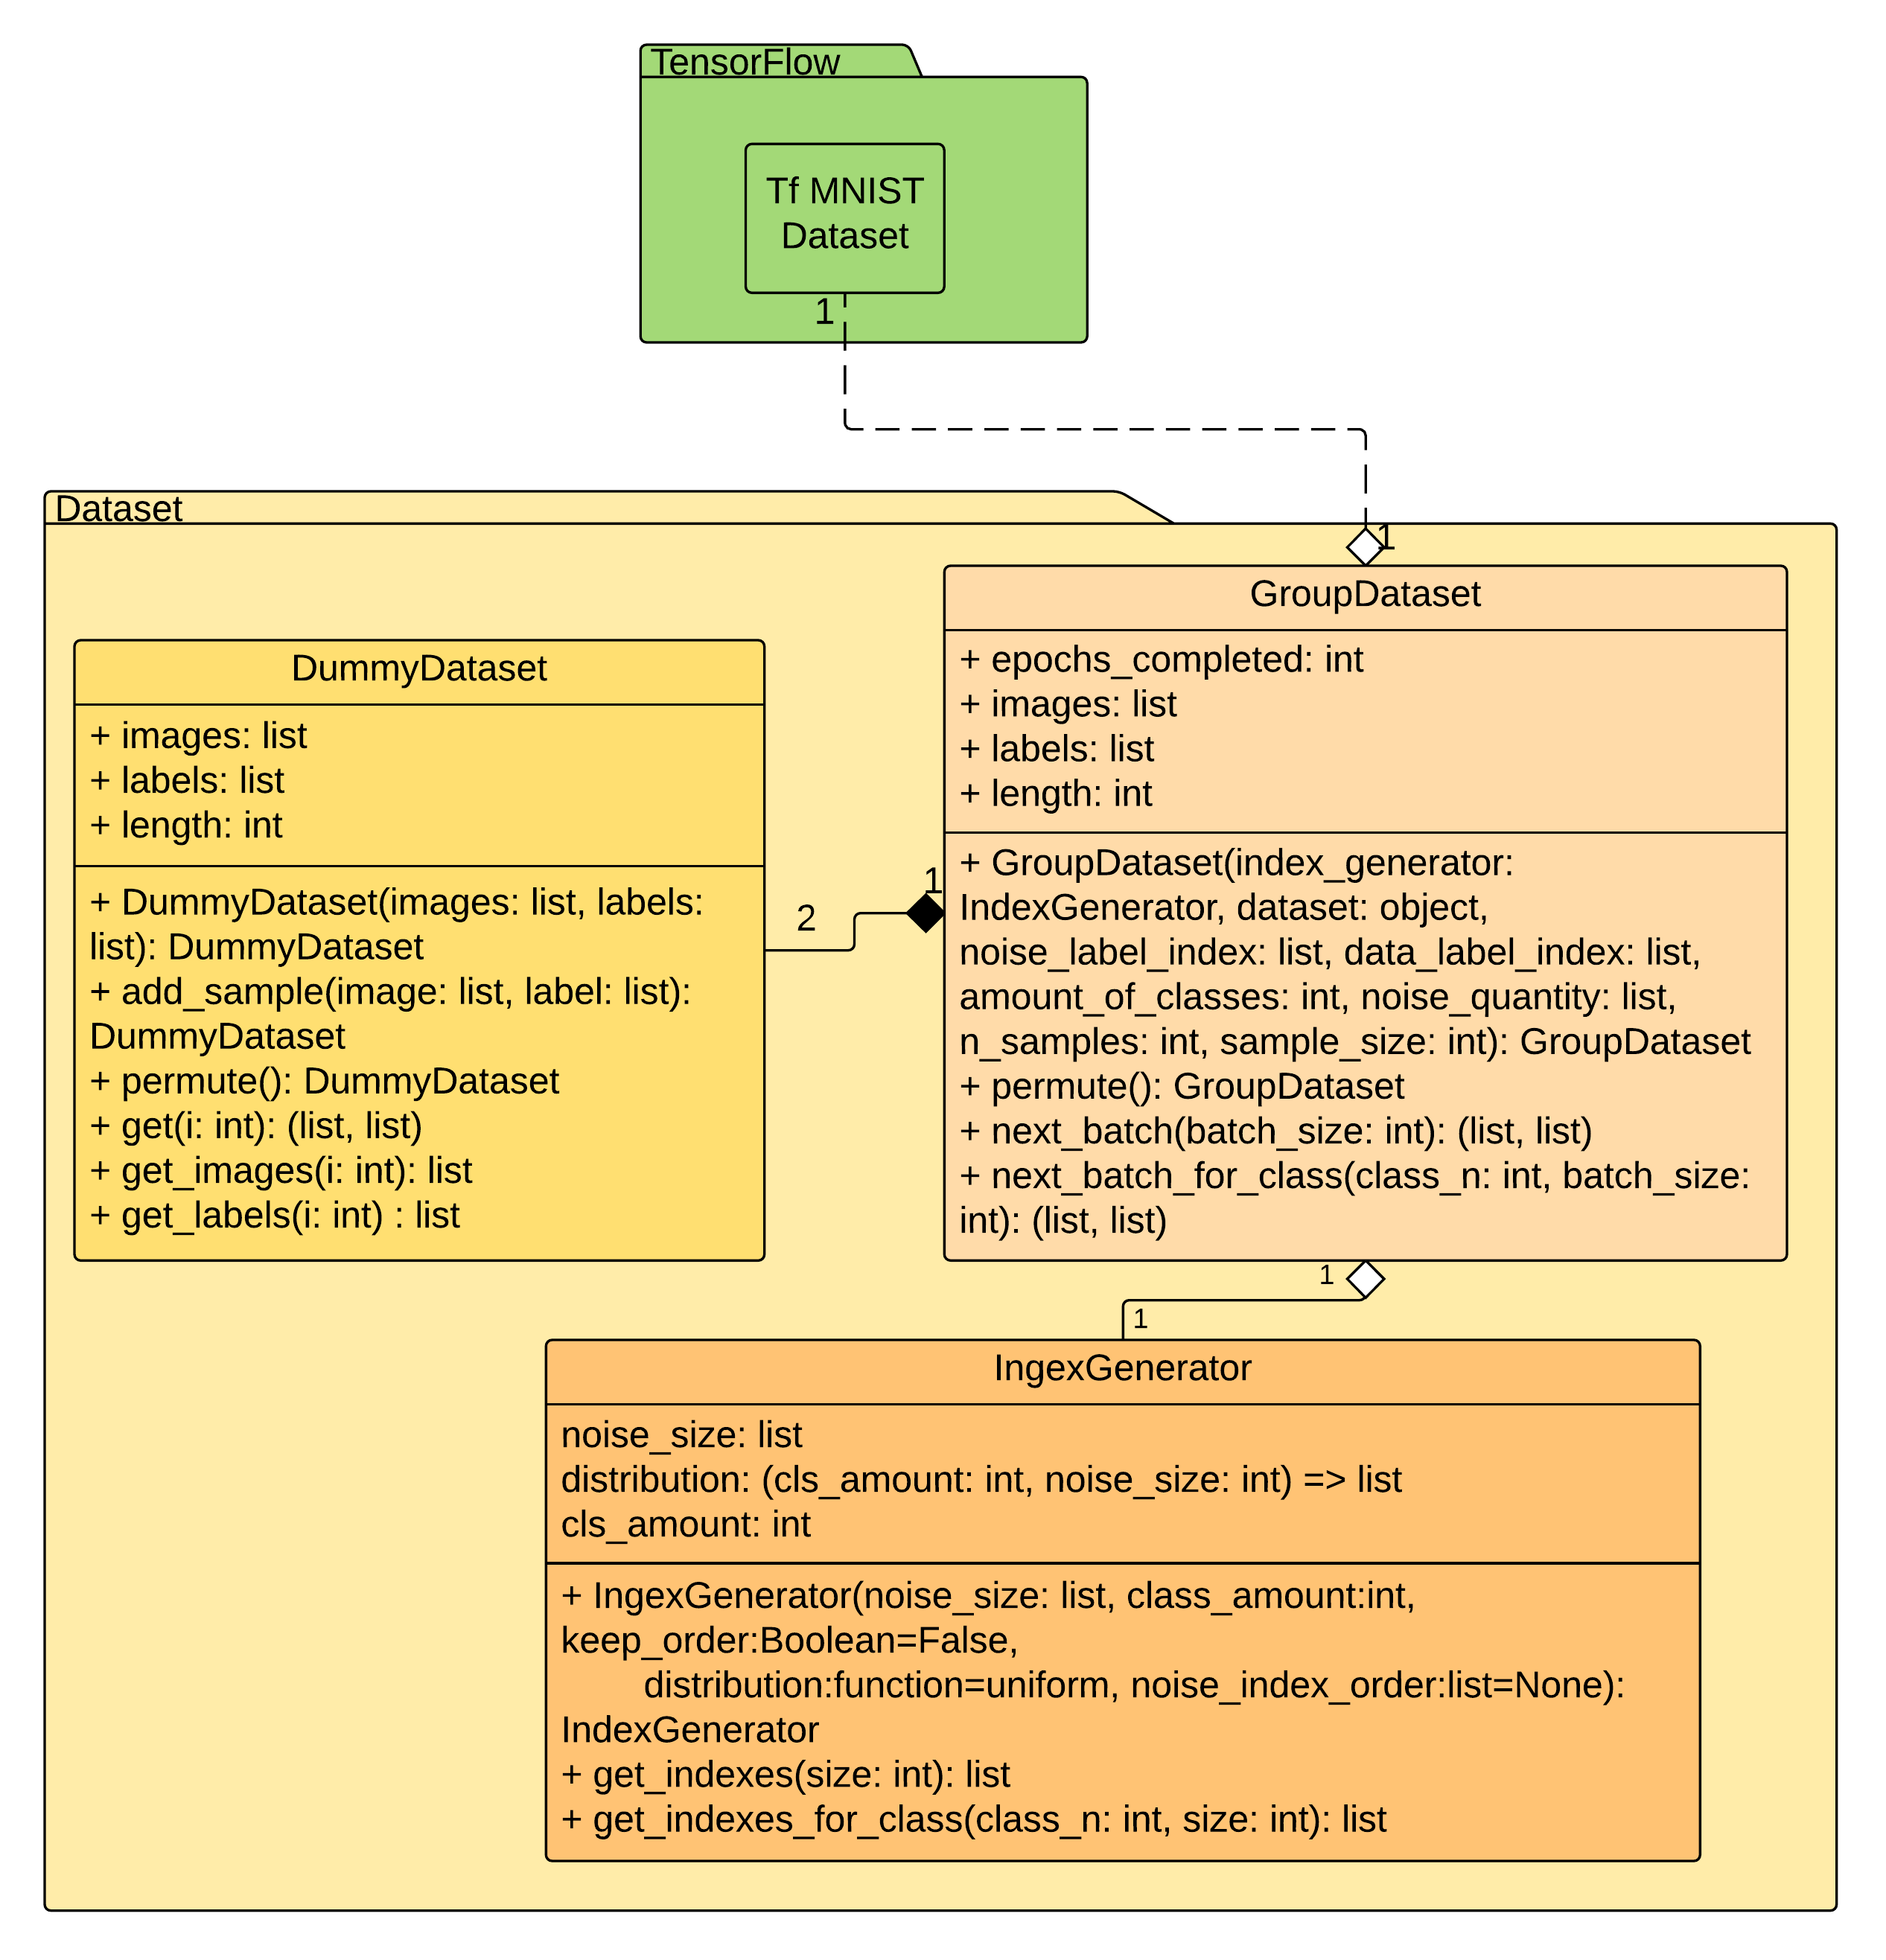
\includegraphics[width=\linewidth]{Dataset_UML}
	\caption{UML class diagram of the dataset module}
	\label{fig:dataset_uml}
\end{figure}

\paragraph{Code pattern} As we can see from the UML class in the figure
\ref{fig:dataset_uml}, we have three classes. It would be also possible
merge the classes, however, this contradicts "Single Responsibility Principle"
that one class should only have one responsibility \cite{martin2003agile}.
Therefore, dividing this into two classes allows us to clearly
define responsibilities. Consequently, this separations seems to be reasonable.

As you might notice from UML class diagram, some of the function like
\lstinline{add_sample} in \lstinline{DummyDataset} returns the object itself: \lstinline{DummyDataset}.
This is an example of Cascade code pattern described in \autoref{sec:quality_concerns}.
% As you might notice from UML class diagram, that \lstinline{GroupDataset} can inherit
% \lstinline{DummyDataset} as they have similar properties,
% but as "Composition over Inhertitance" states, it
% not always a good idea.

%
% inderect variable access. (e.g.)

% TODO:
% look over the Dataset implementation,
% write all documentation
% draw uml diagrams
%
%
%
%
%

% \paragraph{Requirements} Like why do we need index generator
% including flexibility
% \paragraph{Inspiration fromt the tf class dataset}
%
% inpsiration from dataset class from tensor flow: link
% https://github.com/tensorflow/tensorflow/blob/master/tensorflow/contrib/learn/python/learn/datasets/mnist.py
% that should perform similar action to
% The function requirement to the dataset can be formulated as

% \paragraph{
% 	not learning any dependency,
% 	explain that we want to avoid the same samples in a group to avoid that
% }
% model will learn dependency and etc.

% \paragraph{
% 	explain shortly about combinations of MNIST data, how to achieve the best data
% }
%
% \paragraph{then show the uml diagram of dataset}
% including: Class overview
%
% \paragraph{explain what is purpose of each of the class. }


\section{Model}
\label{sec:design_model}

% \paragraph{Why did you choose picker network?}
We described three approaches of how to extend the RAM model
in \autoref{sec:extension}. The implementation of this work
will only concentrate on method described as picker network.
This is because of the simplicity of this approach.

%TODO: patterns https://www.toptal.com/python/python-design-patterns

% \paragraph{about why OO programming is not ALMOST suited and why it should be more functional}
It's common practices in TensorFlow to use functions for implementing the model.
We will stick to this practice for defining the model because this can
potentially reduce the complexity of the model as well as
increase readability of the code.

% \paragraph{The architecture as a whole}

\subsection{Architecture} \label{subs:arch_model} Taking into account
the extension that was
described in \autoref{subs:picker_net}, we can easily derive classes
as each of the networks has a clear task. Building the model will be
possible using following clases:

\begin{itemize}
	\item GlimpseSensor - the class is responsible for extracting glimpses from
		images at given location $l_t$.
	\item PickerNet - the class is responsible for picking an image out of the
		group of images.
	\item GlimpseNet - given the glimpse sensor, images and number of picked image,
		this class is responsible for producing the feature map from the image,
		which is then fed into LSTM cell.
	\item LocNet - the class is responsible for producing next location for
	glimpse sensor to attend to.
	\item Model - formally, this is not a class, but a set of function that build
		and run the model. We will represent this set as a class in UML class diagram
		in \autoref{subs:uml_model}. However, this set of function will also explained
		more detailed in \autoref{subs:model_seq_diagramm}.
		For now we'll refer to it as class.
	\item Config - singleton class that holds all
		configuration parameters for the model such as shape of weights
		for hidden layers.
\end{itemize}


\subsection{UML class diagram}
\label{subs:uml_model}

In the figure \ref{fig:model_uml}, you can see the UML class diagram for the
architecture we described above. As it was already mentioned the \lstinline{Config}
class is a singleton class that holds all configuration details for the model.
Once initialised with command-line options or default values, it's a single source
of true for the whole application. Use of singleton design pattern here helps
to avoid misconception that application can have more than one configuration.
From the UML diagram we see that only class \lstinline{Model} use the
\lstinline{Config}, this is because of the convenience sake. Without much effort
\lstinline{Config} can be imported from other classes as well.

\begin{figure}[H]
	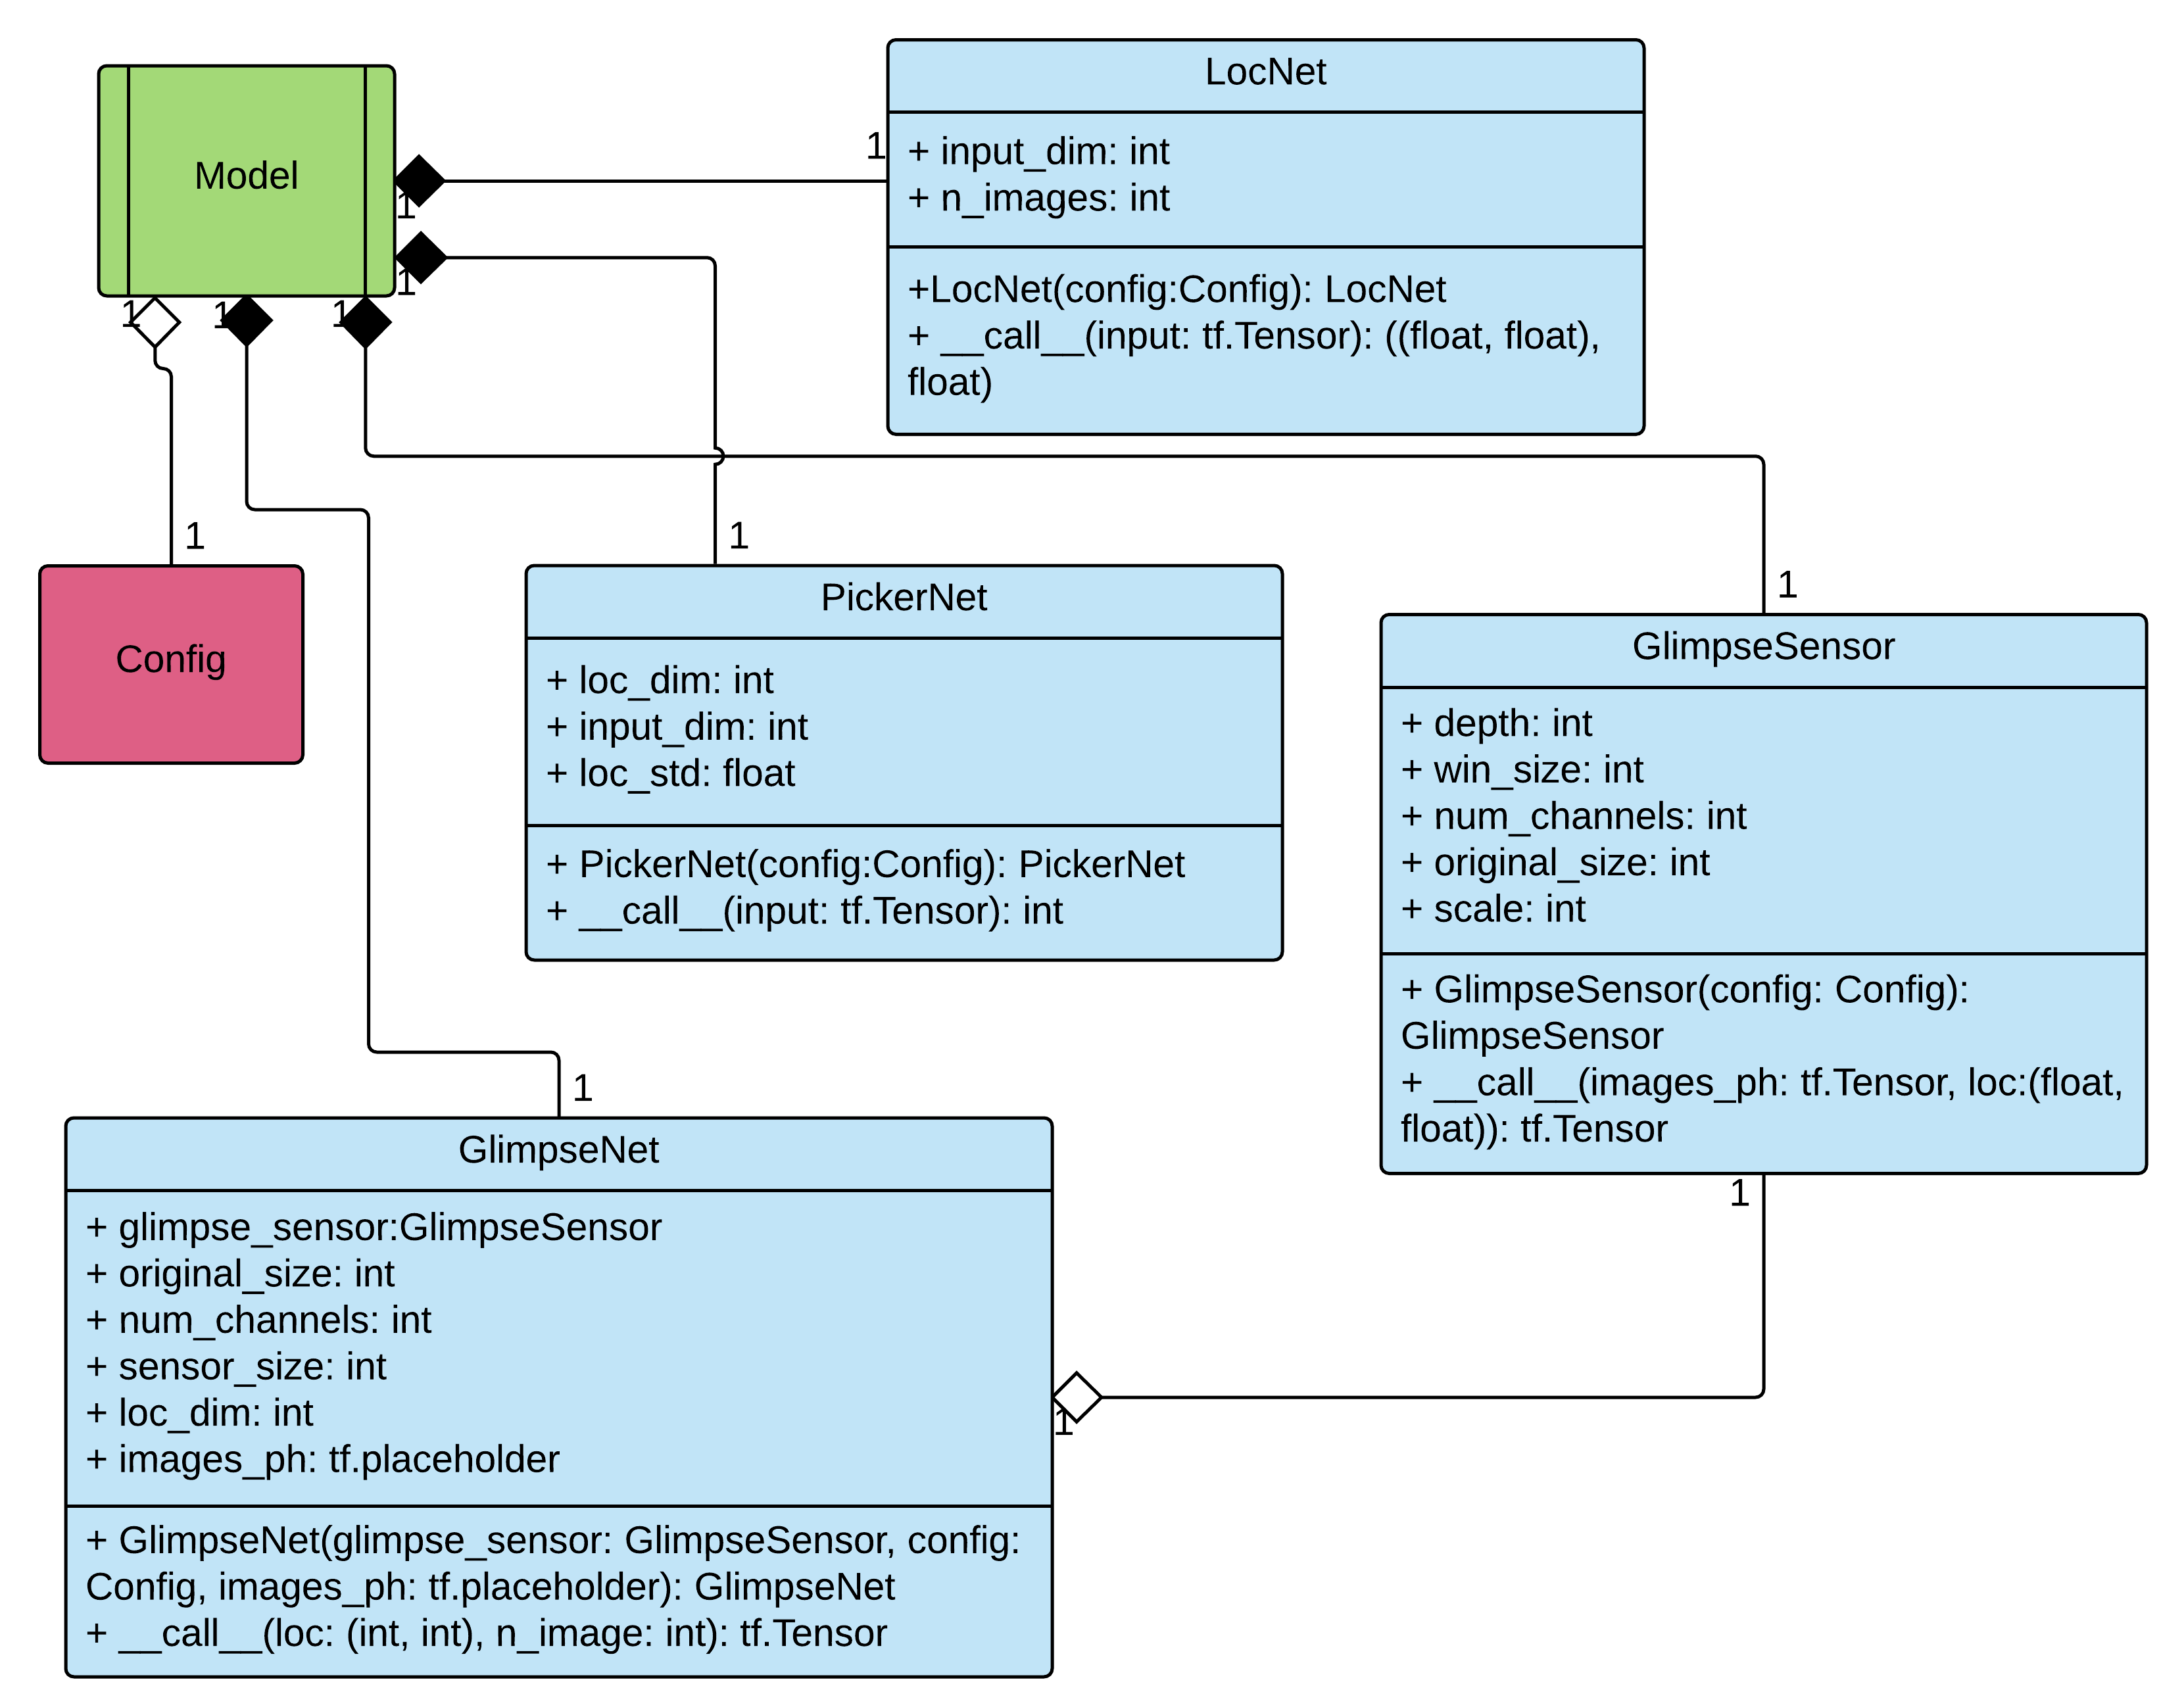
\includegraphics[width=\linewidth]{Model_UML}
	\caption{UML class diagram of the Model component}
	\label{fig:model_uml}
\end{figure}


\subsection{UML activity diagram for the Model}
\label{subs:model_seq_diagramm}
To prevent misunderstanding, we distinguish between \lstinline{Model} class
and Model component. Model component is set of of classes and functions related
to RAM and it's extension. \lstinline{Model} class is a class that we described
in \autoref{subs:arch_model}.
As it was mentioned earlier, the \lstinline{Model} is not an actual class, but a set of
function. \lstinline{Model} class is core of the Model component. It instantiates
other classes as well as runs, trains
and evaluates the model. Since then \lstinline{Model} is contains only functions,
it's hard to represent it as UML class diagram. However, UML activity diagram
can be a good fit if we replace the activities in the UML notations with
the functions. Therefore to clarify the flow of the \lstinline{Model}, you may
find the figure \ref{fig:uml_activity_model} with the UML activity diagram helpful.
In the lane with the name \lstinline{init_seq_rnn()}, you can see a set of functions
related to LSTM cell initialisation. This lane means that inside \lstinline{init_seq_rnn()}
function this set of function is called.
The container with the name "calculate the hybrid loss", mean nothing more than
conceptual conncetion between the function inside.
We will take a closer look at some of details of this functions in the
\autoref{ch:implementation}.
% As you can see from the diagrams, the functions names can describe the
% functionality that it does. With
% \label{sec:quality_concerns}


%  To get an idea of what \lstinline{Model} does,
%
% To simplify the understanding of what the \lstinline{Model}
% consist


\begin{figure}[H]
	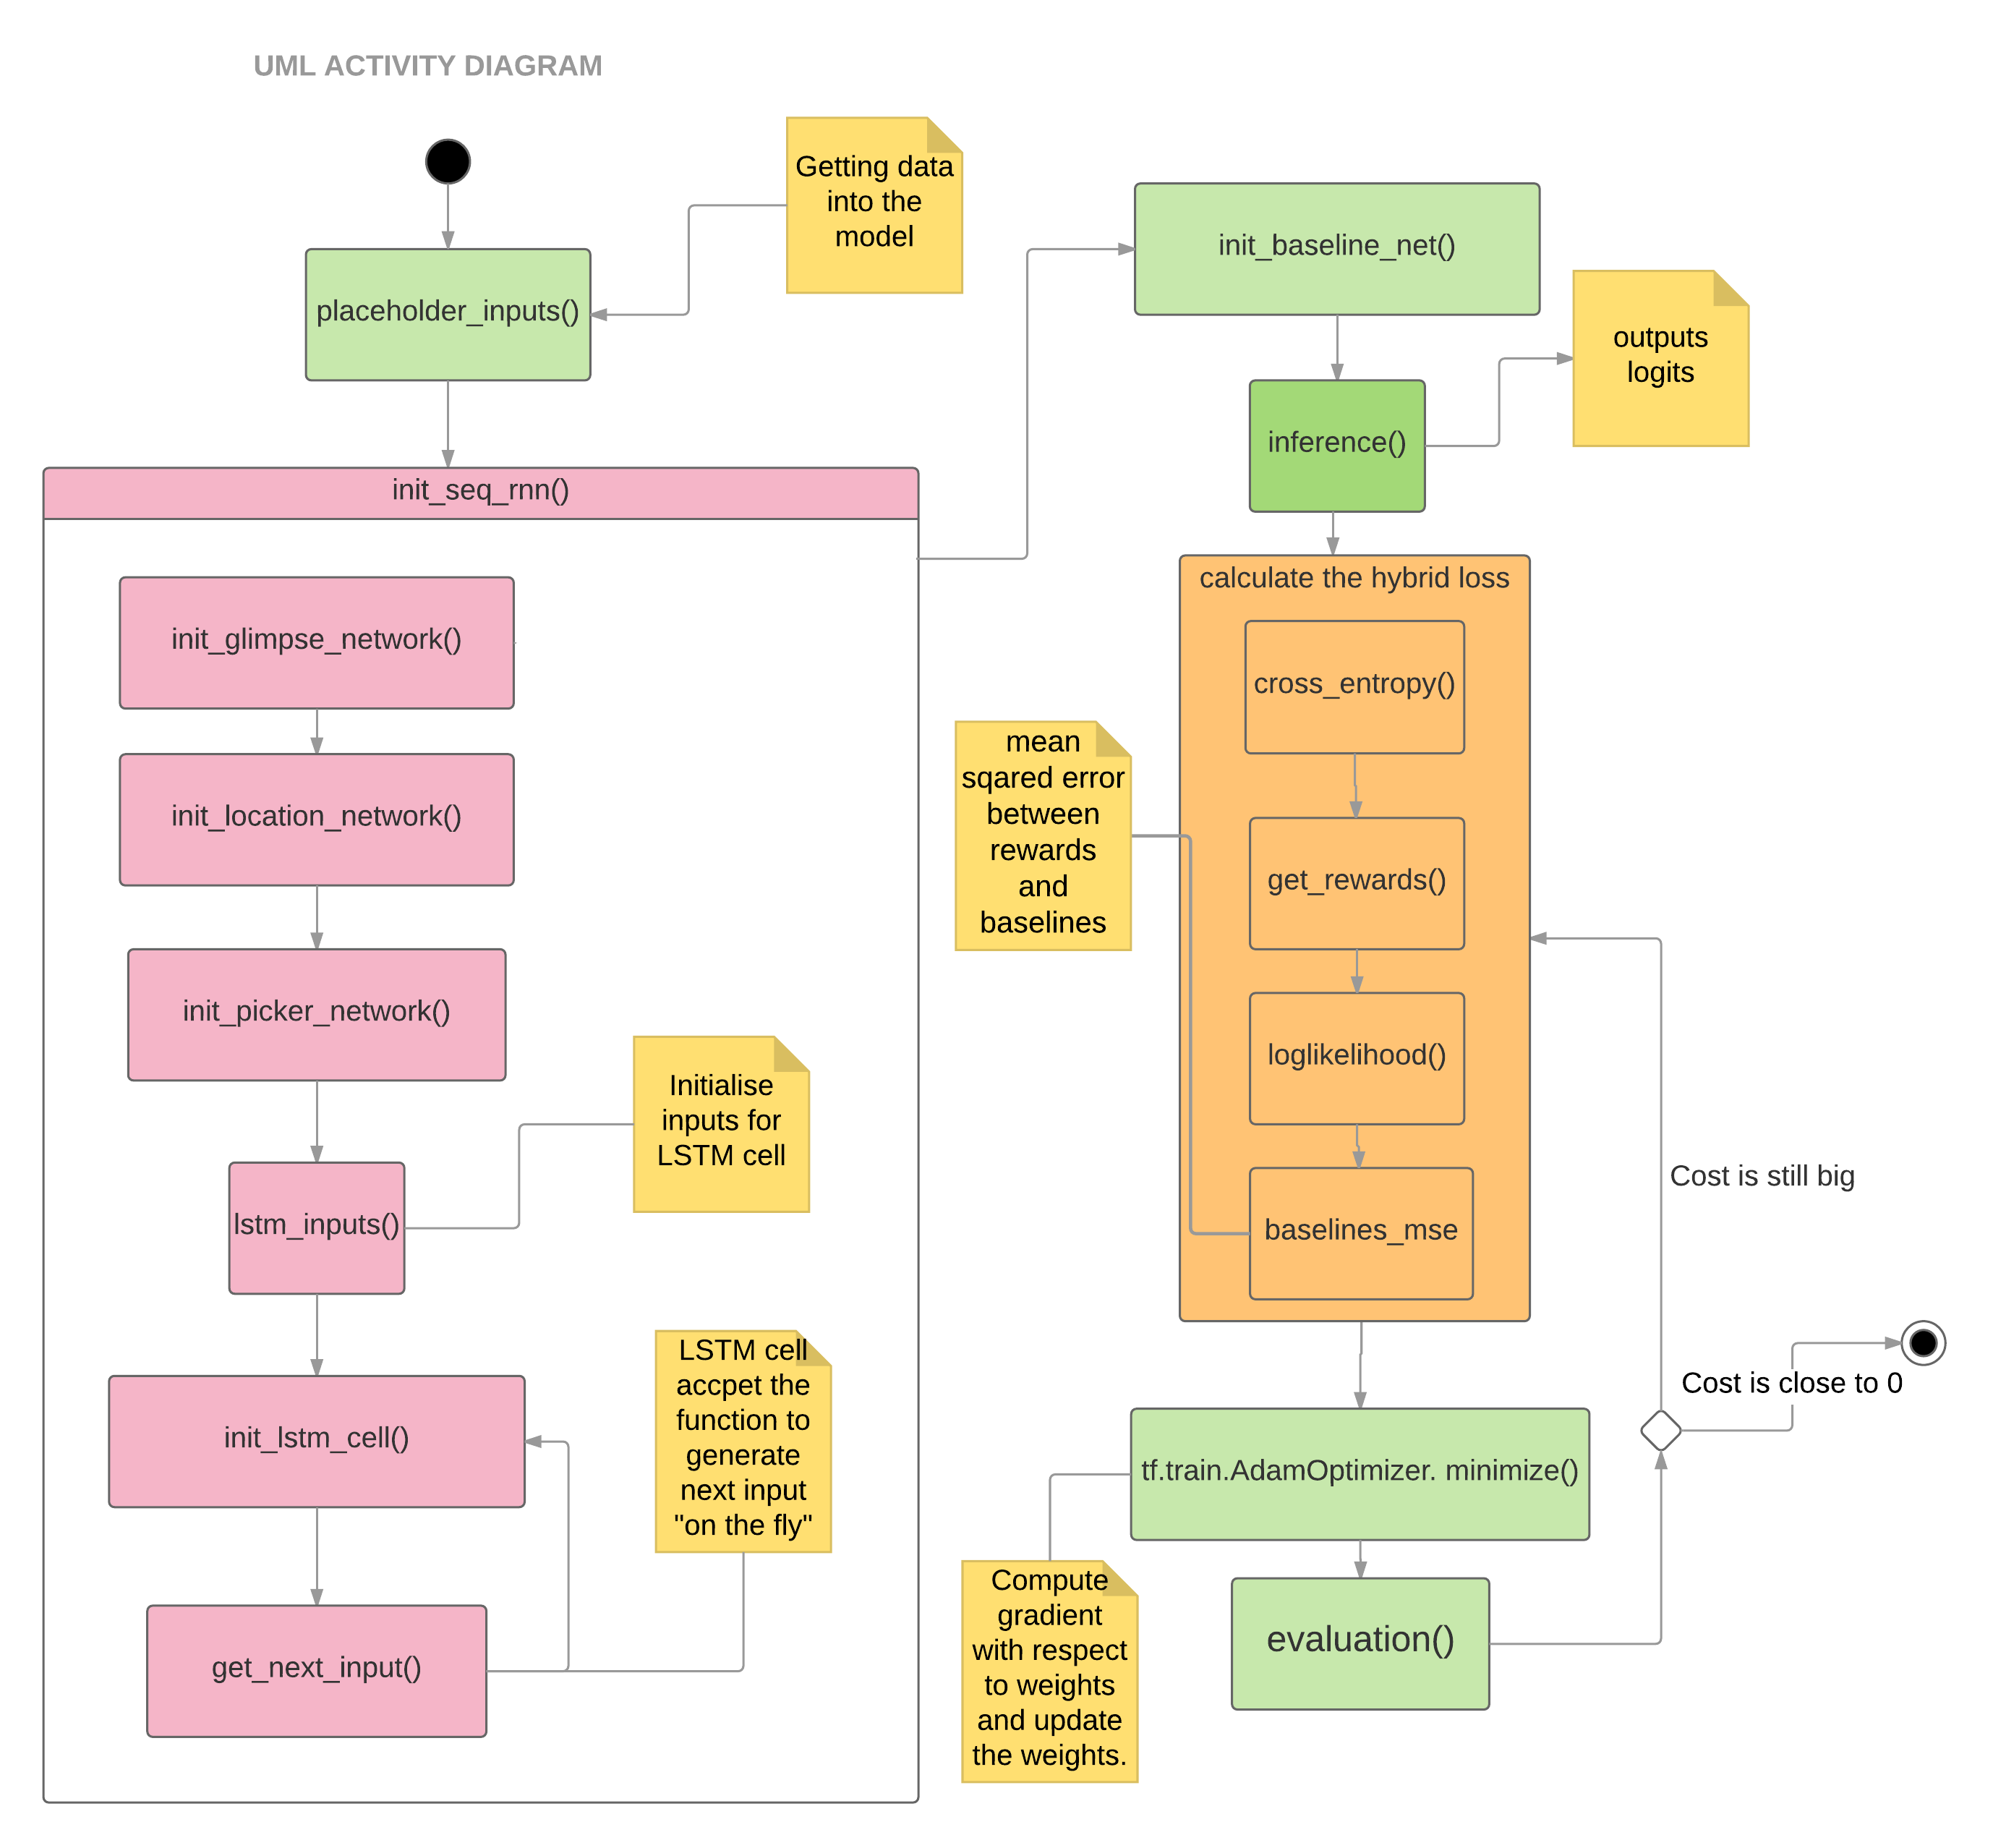
\includegraphics[width=\linewidth]{uml_activity_model}
	\caption{UML activity diagram of the Model}
	\caption*{This is simplified flow of the \lstinline{Model} class.
	Each activity represent a function. For the sake of simplicity some of the function
	are not shown here. However, it should not influence on the understanding
	of the \lstinline{Model}}.
	\label{fig:uml_activity_model}
\end{figure}
%
% #
% Sequence:
% input(images)
% Init RNN ->
%     init_glimpse_network
%     init_location_network
%     init_picker_network
%     init lstm_inputs
%     init LSTM cell
%     defined the next input function for LSTM (get_next_input) --> depends on the all above
%     -> outputs
% init_baseline_net(outputs)
% cross_entropy(logits, groud_truth)
% get_rewards(pred_labels, labels_ph) --> calculate rewards
% define loglikelyhood ratio
% defined hybrid loss
% train the model with AdamOptimizer with respect to loss.
% #
% the plan:
% draw uml diagram: represent the main run_training as a class.
% make a note that it's actually not a class but a set of functions to
% to represent the model.
% then draw this main class again with the explanation of how the
% things is working using any sequential type of diagram.
% Config is singleton
% \paragraph{Possible classes, overview}
% \paragraph{UML diagram}
% \paragraph{back up the classes with design patterns}
%
% \paragraph{the flow of the data via function}


% \subsection{Configuration of the project, what can be configured, the complexity of the model}




% write about configuration file in implementation
% the curent desing is using the approach
% described in \autoref{ssec:picker_net}.
%
% Basically explain the flow of input data, all losses, and baselines, and etc.
% if there is anything relative to the structure in the code use the references to the design patters
% Show all classes, write the documentation for those, or at least briefly explain the purpose.
% The process of training, maybe explain the whole idea behind this
% 	seperation of dataset into validation, test, training.
% look at the other bachelorarbeits and look of what they wrote there
% think about whether it's possible to combine the design and implemntation chapters
%
%
%
% * Entwurfsstrategie, Beschreibungen funktionaler und nich
%  funktionaler Anforderungen, Einsatz von Mustern und
%  Bibliotheken, Softwarearchitektur, Verwendung von Datentypen und
%  Datenstrukturen, Algorithmen, Mensch-Maschine-Schnittstelle;

    \chapter{Design}
\label{ch:implementation}


\section{TensorFlow}
\paragraph{How the computation works in tensorflow, sessions}
\paragraph{How the data coming in --> Placeholders}

\paragraph{what is tensor}
\paragraph{what is ops}

\section{Code quality}

\subsection{Patterns}
\paragraph{Documentation}
\paragraph{Naming, Code readability}

\section{Details}
\paragraph{what is hybrid loss}
\paragraph{How the loss is calculated}
\paragraph{How the baseline is calculated}
\paragraph{How the rewards are calculated}
\paragraph{
	the way the optimizer works, like all variables get updated and
	why should we use stop_gradient
}

    \chapter{Test and evaluation}
In this chapter, we will discuss how the testing is done
in the implementation of this work as well as how
the current model was evaluated.
\section{Test}
In the current implementation, we test our prototype by the means
of unit testing. Unit testing is a method of software testing,
which verifies that individual units of the code are working
as expected. To perform the unit testing, one should identify
pieces of code, that are responsible for a clear task \cite{Huizinga2007}.
In most cases,
that are methods of classes or functions. Imagine, that we have
a function that adds two numbers together. To test this function,
we have to come up with the real values, calculate the expected
return, call the function with the real value and compare
the return of the function with the expected return:

\begin{lstlisting}[language=Python, caption={TensorFlow example \cite{tensorflow2015-whitepaper}},label={list:test_ex}]

	def add(x, y):
		"""Add two numbers together."""
		return x + y

	# unit test of the function `add`
	def test_add():
		assert add(3, 5) == 8 # 3, 5 are real values, 8 is the expected return
		assert add(10, 2) == 12
\end{lstlisting}

In case of classes, mostly it's methods were covered with unit tests.
For testing purposes, we
used unit test framework called Nose. Nose simplifies unit testing
by providing automatic test discovery. It also automatically creates a test suite,
which is nothing more than a set of tests. One advantage of using the Nose
over the Python’s standard unit test module is that no configuration is required
in order to run all tests when the tests are named consistent with Nose conventions
and are located in the \emph{/tests} directory. An additional advantage is that
Nose generates well-readable report after running tests. The report helps
when debugging and fixing tests. You can see the example of an report on the figure
\ref{fig:report_test}

% TODO: two figures from the command line
\begin{center}
	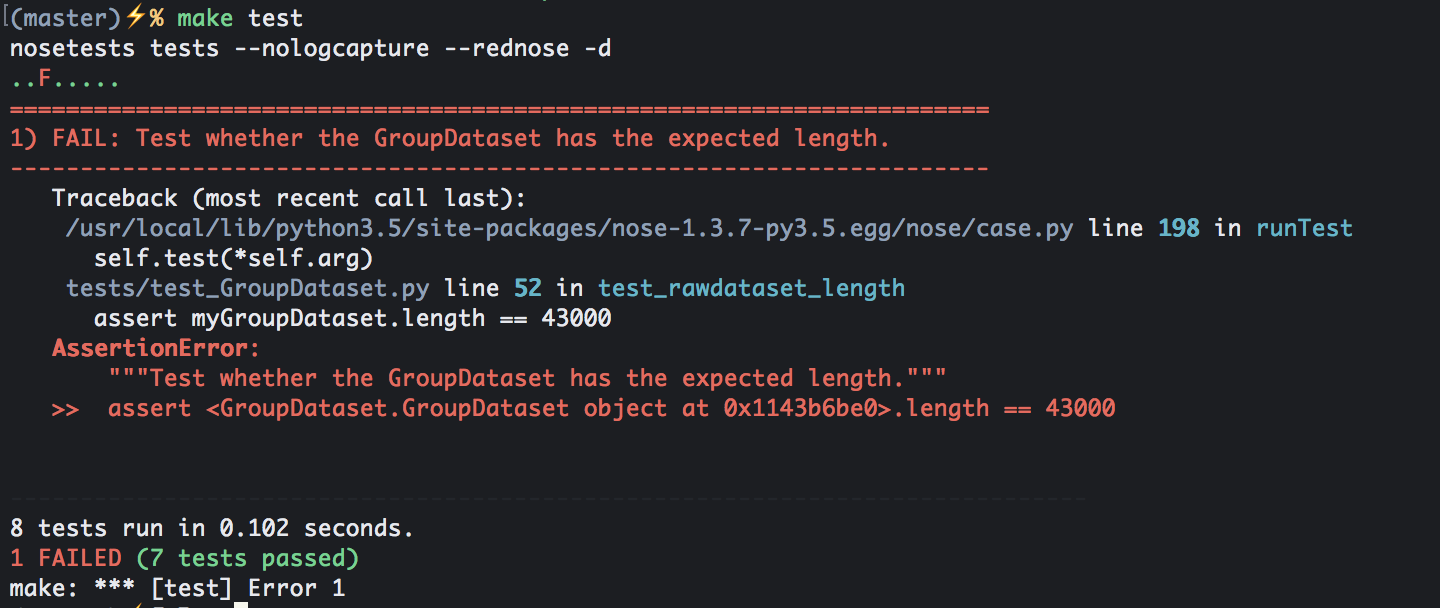
\includegraphics[width=\linewidth]{test_report}
	\caption{Output of executing command \lstinline{make test} in the root of the prototype
		with a failing test.
	}
	\label{fig:report_test}
\end{center}

\subparagraph{} The module Dataset is fully tested with unit tests. However,
the module Model is not, since it has too many non-deterministic values.
One good way of testing the model is to run an interactive session of TensorFlow,
which is desired for the further development of the prototype.\footnote{
TensorFlow documentation explains this method here: https://www.tensorflow.org/api_guides/python/test
}

\section{Evaluation} The model was evaluated with the dataset described
in \autoref{sec:analysis_dataset} on server from HTW Berlin. The server
posses the Nvidia Tesla M40 GPU accelerator \cite{NVIDIA}.
It was required from 1 to 2 hours to train the model and the time is changed
caused by different configurations.
We will introduce more details of the first experiments below in this section.

\subsection{Configuration}
The evaluation was performed on two different types of setting.
You can see the differences between these configurations
in table \ref{tab:conf_exp}.

We will explain the settings that are different in the configurations:
\begin{itemize}
	\item Number of glimpses($T$) - As you can remember from \autoref{sec:ram_model}
	the agent does a classification decision after $T$ steps. In original RAM
	paper this number was equal to $T=7$. Since we will have more images in a group,
	we increased this number in both of configurations.
	\item Batch size - size of the batch for training the model.
	\item Labels of noise pictures - the images at the labels considered to be
	 	insignificant for the classification decision(as described in \autoref{sec:analysis_dataset}).
	\item Labels of non-noise pictures -  the image at the labels are important
		for the classification(as described in \autoref{sec:analysis_dataset}).

	\item Amount of images per group - this amount determines how many images
	a group will have.
	\item Amount of classes for classification task - as you may remember from
		\autoref{sec:analysis_dataset}, we can build dataset with different
		amount of classes.
\end{itemize}

\begin{table}[]
\centering
\resizebox{\textwidth}{!}{%
	\begin{tabular}{|l|l|l|l|}
	\hline
	Name of the parameter                     & Configuration 1        & Configuration 2           & Configuration 3           \\ \hline
	Batch size                                & 32                     & 20                        & 20                        \\ \hline
	Number of glimpses ($T$)                    & 30                     & 15                        & 24                        \\ \hline
	Labels of  noise pictures                 & 1,2                    & 0                         & 0                         \\ \hline
	Labels of non-noise pictures              & 0, 3, 4, 5, 6, 7, 8, 9 & 1, 2, 3, 4, 5, 6, 7, 8, 9 & 1, 2, 3, 4, 5, 6, 7, 8, 9 \\ \hline
	Amount of images per group                & 5                      & 5                         & 4                         \\ \hline
	Amount of classes for classification task & 3                      & 3                         & 2                         \\ \hline
	Amount of examples in training dataset    & 45000                  & 45000                     & 60000                     \\ \hline
	\end{tabular}
}
\caption{Configurations for the experiments}
\label{tab:conf_exp}
\end{table}

These configurations was a try to simplify the task for the model. From configuration 1
to configuration 3, we reduced training batch size, reduced the variety of the noise images,
reduced amount of classes, and played with number of glimpses.

\subparagraph{}
Of course, there even more parameters that is possible to tune
in further experiments. The explanation of all parameters can be found
in the implementation of the model.

\subsection{Results}
Generally speaking, the experiments highlighted that the model is not able
to generalise on the validation as well as on the test data.
We will show the evidence of that by referring to the figures taken from
TensorBoard.
The figures \ref{fig:valid_accuracy} and \ref{fig:test_accuracy} indicate that the accuracy on the validation
and test data weren't stable. The training accuracy for all three configurations
was stable and reached high results as shown in the figure \ref{fig:batch_accuracy}.
Proceeding from that, we can state that overfitting occurs
by training the model.

\begin{figure}
\centering
\begin{subfigure}{\textwidth}
  \centering
  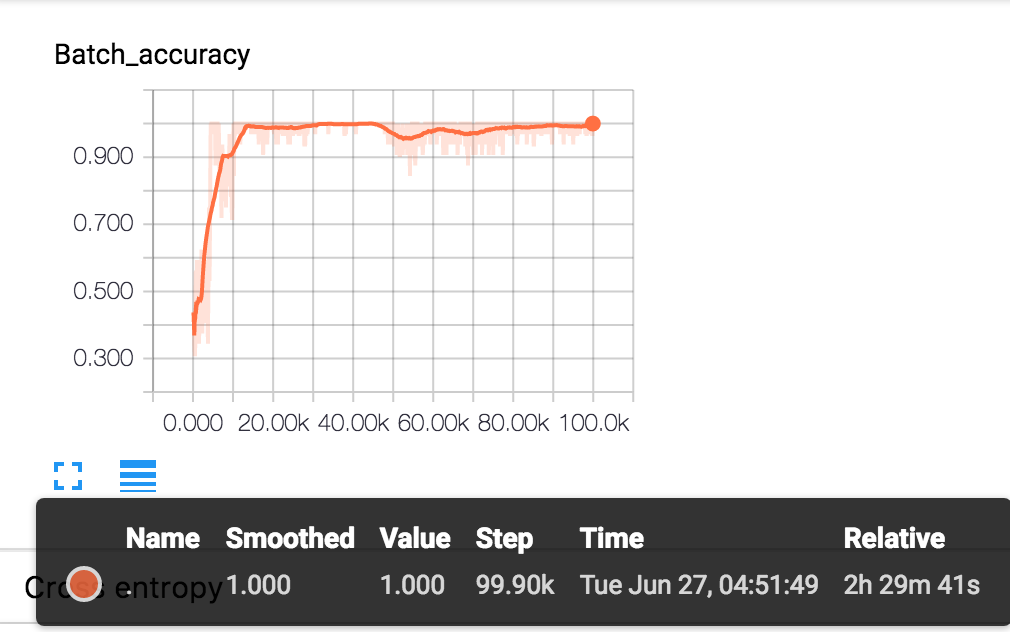
\includegraphics[width=0.8\linewidth]{config1/batch_accuracy}
  \caption{Configuration 1}
  % \label{fig:b_acsub1}
\end{subfigure}
\begin{subfigure}{\textwidth}
  \centering
  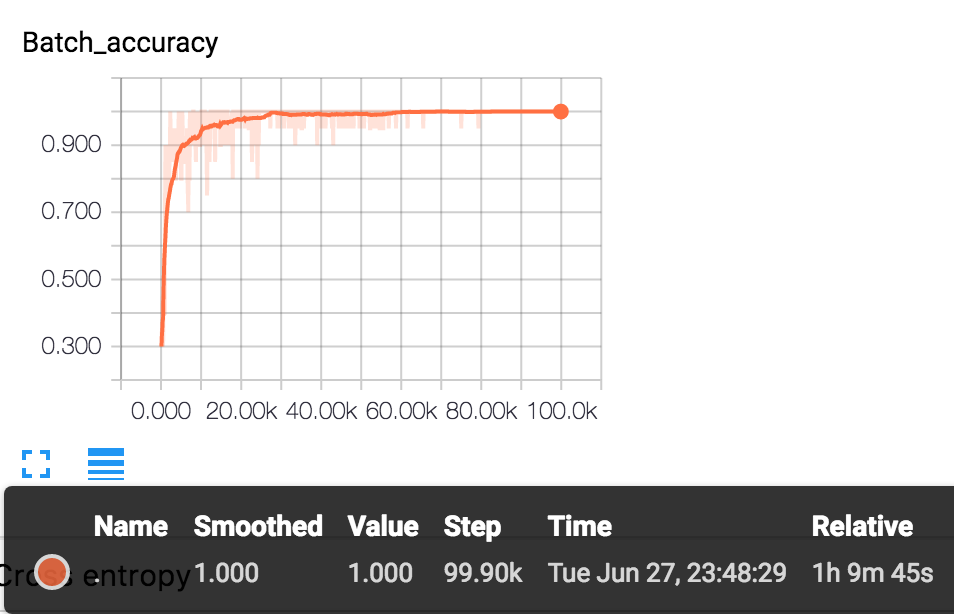
\includegraphics[width=0.8\linewidth]{config2/batch_accuracy}
  \caption{Configuration 2}
  % \label{fig:sub2}
\end{subfigure}
\begin{subfigure}{\textwidth}
  \centering
  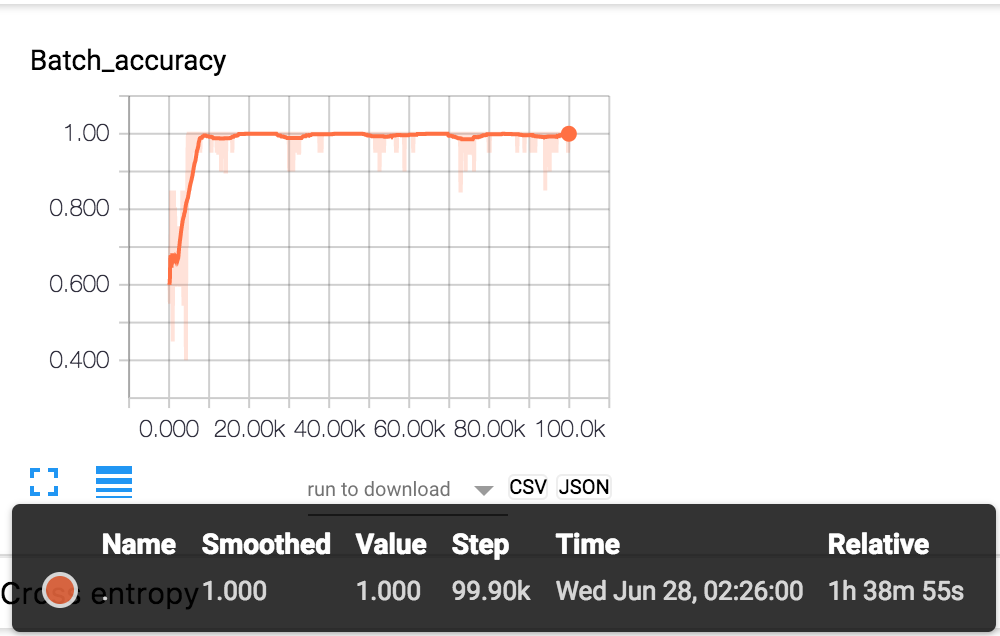
\includegraphics[width=0.8\linewidth]{config3/batch_accuracy}
  \caption{Configuration 3}
  % \label{fig:sub2}
\end{subfigure}
\caption{Accuracy on the training data}
\label{fig:batch_accuracy}
\end{figure}


\begin{figure}
\centering
\begin{subfigure}{\textwidth}
  \centering
  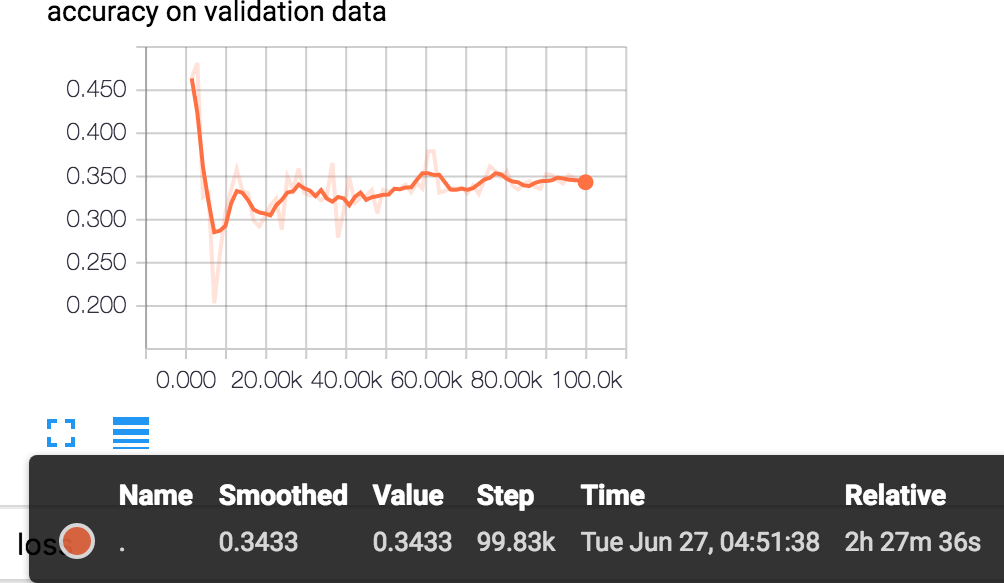
\includegraphics[width=0.75\linewidth]{config1/valid_accuracy}
  \caption{Configuration 1}
  \label{fig:sub1}
\end{subfigure}
\begin{subfigure}{\textwidth}
  \centering
  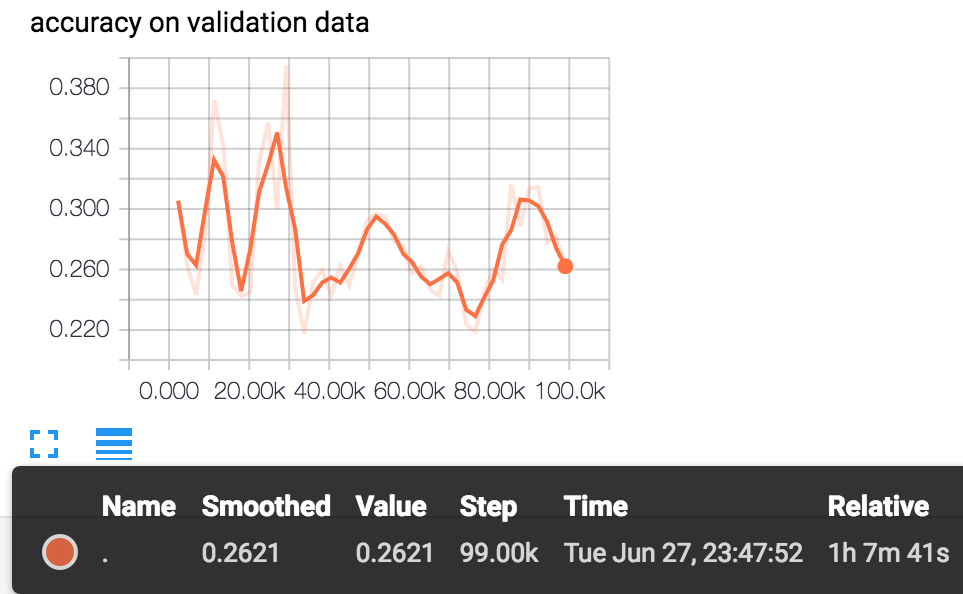
\includegraphics[width=0.75\linewidth]{config2/valid_accuracy}
  \caption{Configuration 2}
  \label{fig:sub2}
\end{subfigure}
\begin{subfigure}{\textwidth}
  \centering
  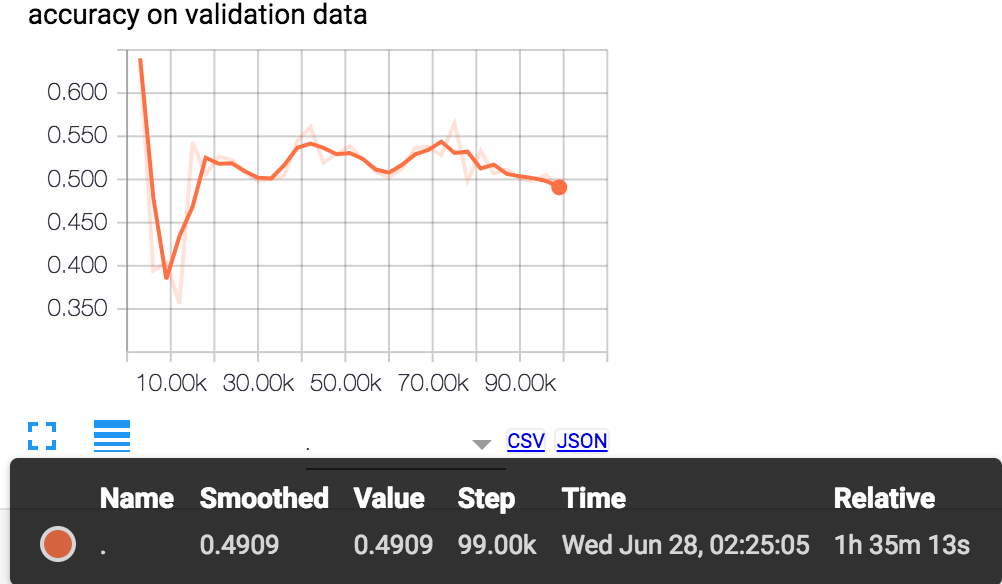
\includegraphics[width=0.75\linewidth]{config3/valid_accuracy}
  \caption{Configuration 3}
  \label{fig:sub2}
\end{subfigure}
\caption{Accuracy on the validation data}
\label{fig:valid_accuracy}
\end{figure}


\begin{figure}
\centering
\begin{subfigure}{\textwidth}
  \centering
  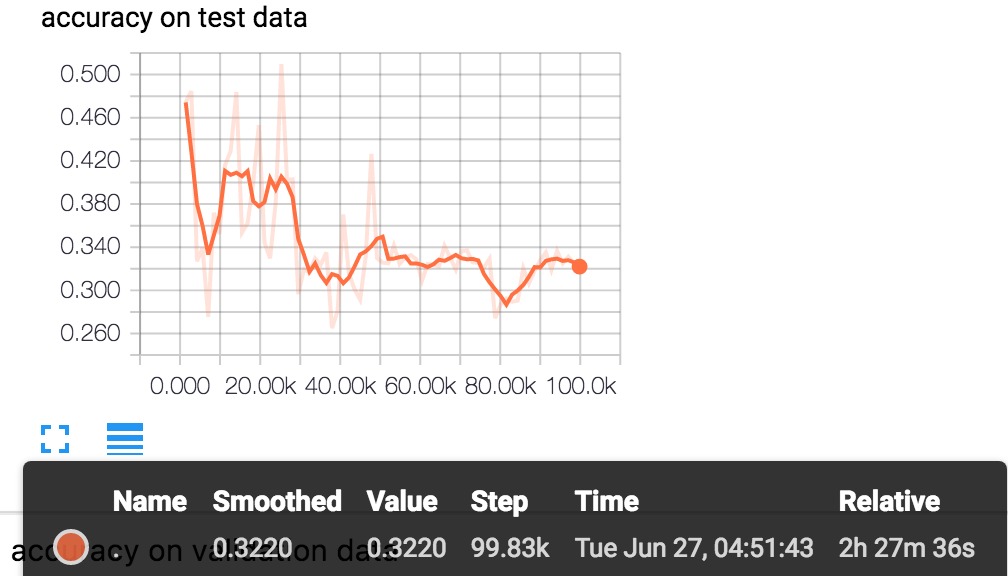
\includegraphics[width=0.75\linewidth]{config1/test_accuracy}
  \caption{Configuration 1}
  \label{fig:sub1}
\end{subfigure}
\begin{subfigure}{\textwidth}
  \centering
  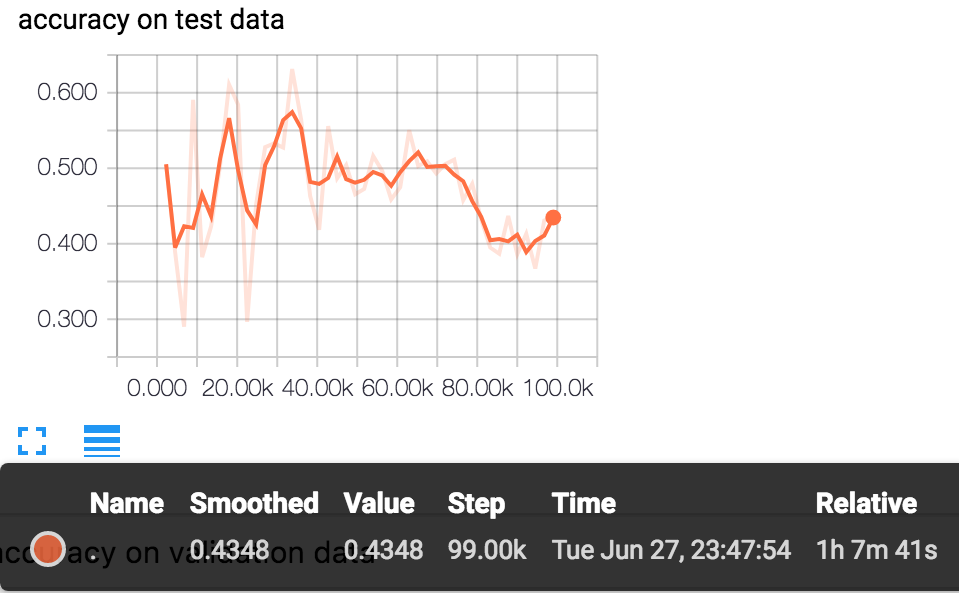
\includegraphics[width=0.75\linewidth]{config2/test_accuracy}
  \caption{Configuration 2}
  \label{fig:sub2}
\end{subfigure}
\begin{subfigure}{\textwidth}
  \centering
  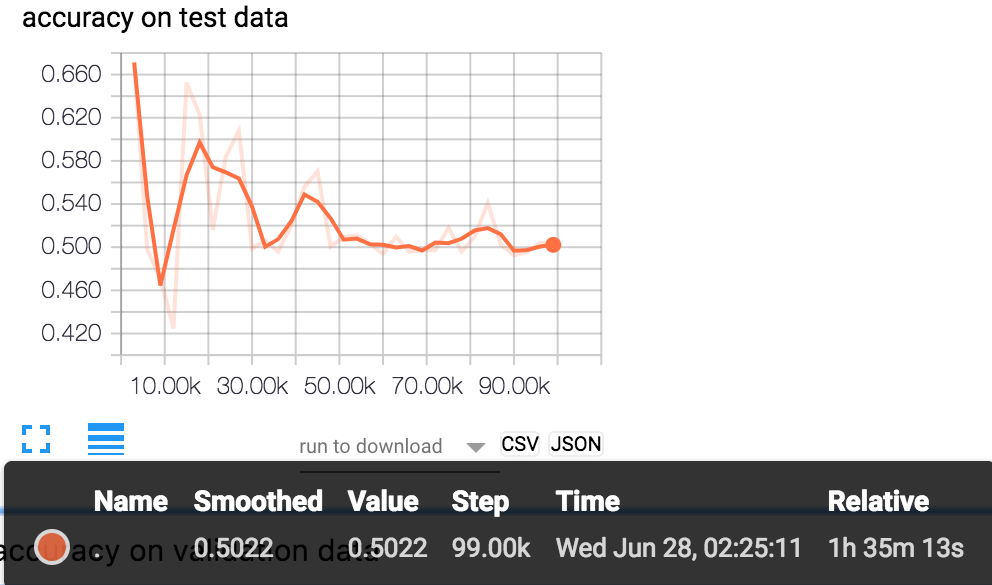
\includegraphics[width=0.75\linewidth]{config3/test_accuracy}
  \caption{Configuration 3}
  \label{fig:sub2}
\end{subfigure}
\caption{Accuracy on the test data}
\label{fig:test_accuracy}
\end{figure}

The figure \ref{fig:baseline_mse} shows that the mean squared error between our value function
for reducing the variance and actual reward is very small. This may indicate, that
the our baseline function is close to the actual expected reward.

Average reward value showed that agent was performing good and
in average was choosing the right actions. The evidence of that is
shown in the figure \ref{fig:average_reward}.
\begin{figure}
\centering
\begin{subfigure}{\textwidth}
  \centering
  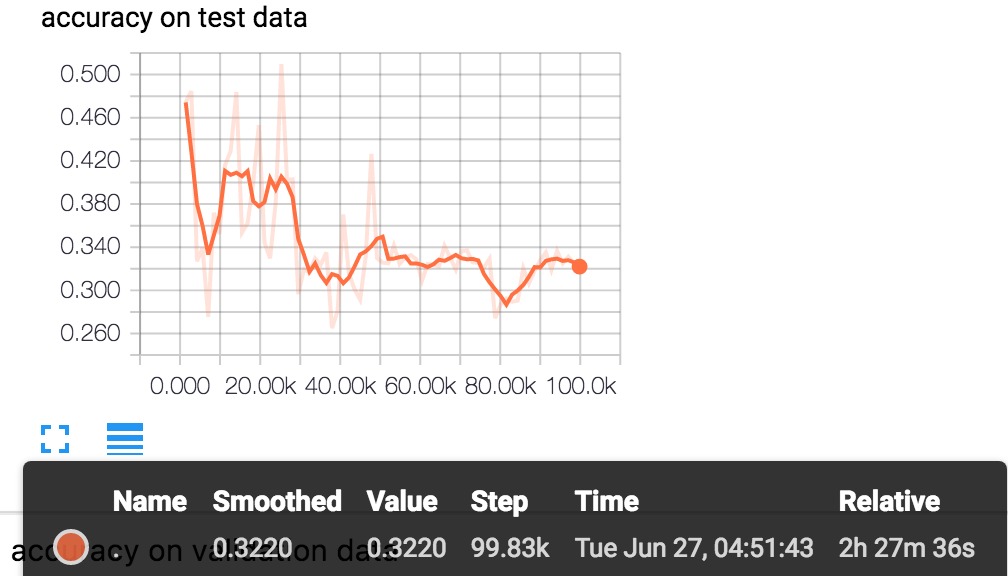
\includegraphics[width=0.75\linewidth]{config1/test_accuracy}
  \caption{Configuration 1}
  \label{fig:sub1}
\end{subfigure}
\begin{subfigure}{\textwidth}
  \centering
  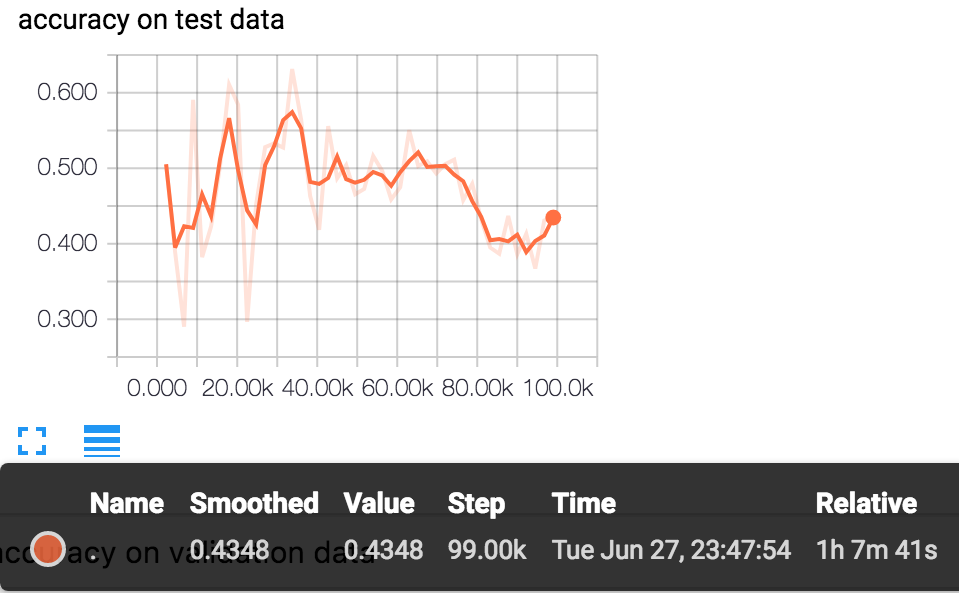
\includegraphics[width=0.75\linewidth]{config2/test_accuracy}
  \caption{Configuration 2}
  \label{fig:sub2}
\end{subfigure}
\begin{subfigure}{\textwidth}
  \centering
  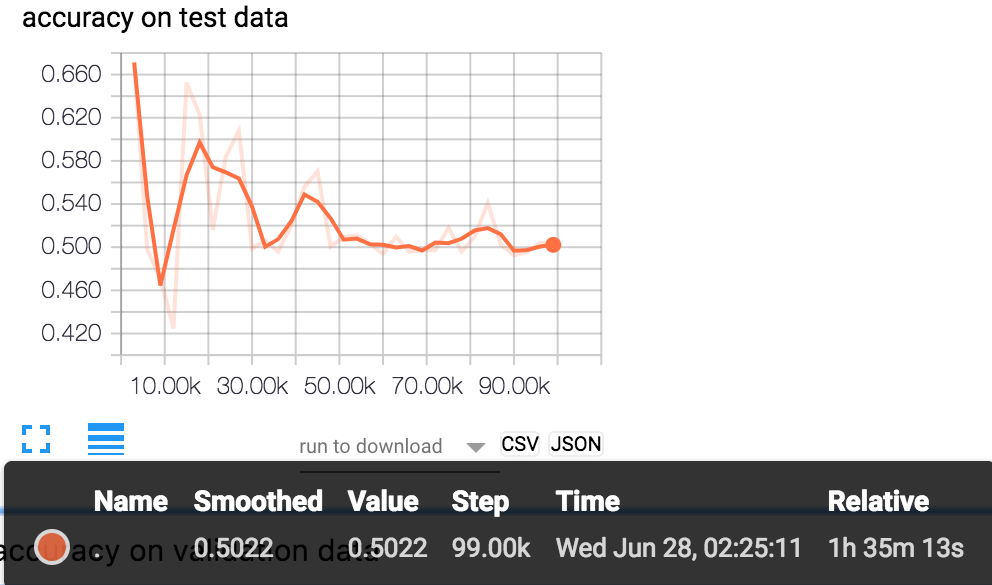
\includegraphics[width=0.75\linewidth]{config3/test_accuracy}
  \caption{Configuration 3}
  \label{fig:sub2}
\end{subfigure}
\caption{Mean squared error between baseline function and expected reward}
\label{fig:baseline_mse}
\end{figure}

From the figure \ref{fig:hybrid_loss}, we can observe the hybrid loss value reduced much more in
the  configuration 3. The reason for this can be, that we reduced the amount
of classes from 3 to 2.
\begin{figure}
\centering
\begin{subfigure}{\textwidth}
  \centering
  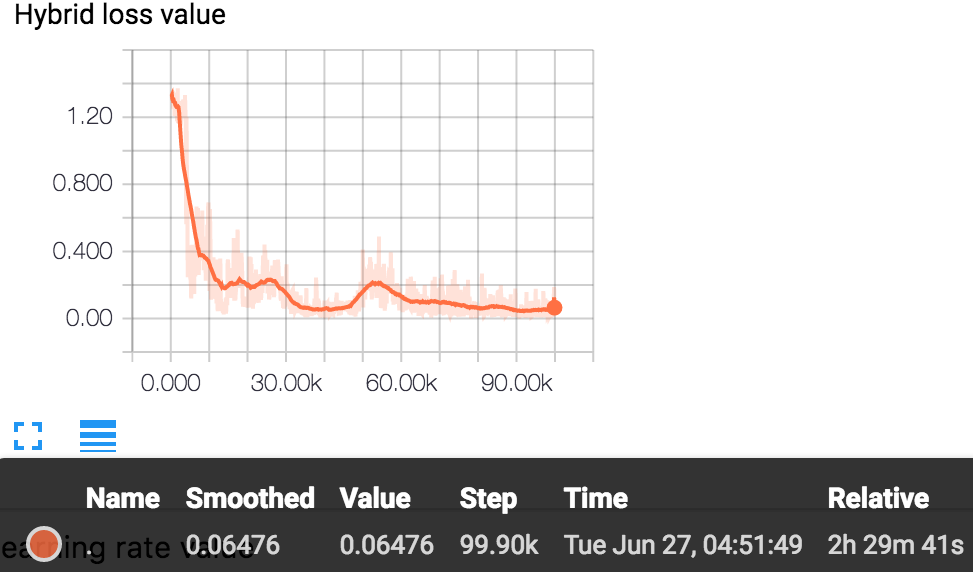
\includegraphics[width=0.75\linewidth]{config1/hybrid_loss}
  \caption{Configuration 1}
  \label{fig:sub1}
\end{subfigure}
\begin{subfigure}{\textwidth}
  \centering
  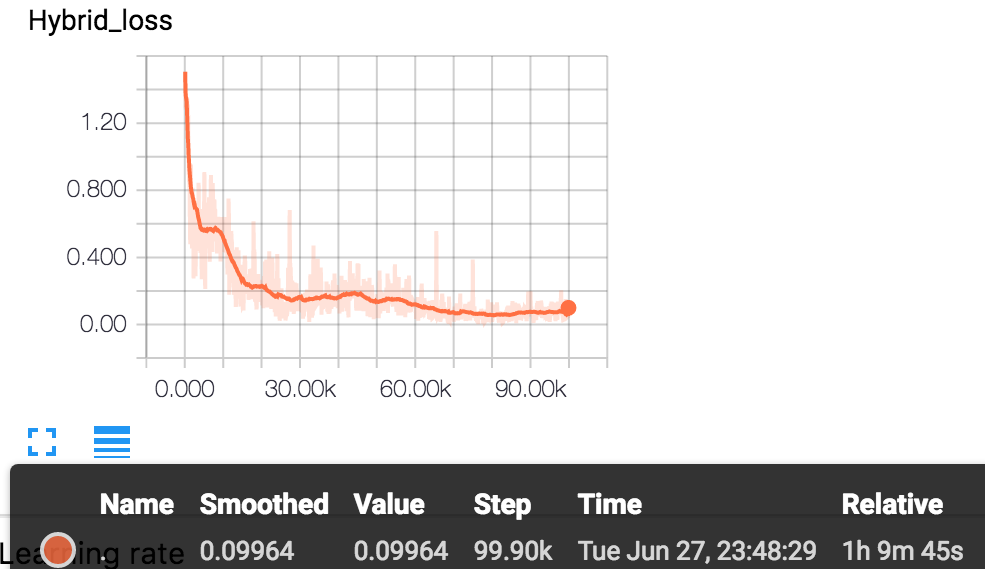
\includegraphics[width=0.75\linewidth]{config2/hybrid_loss}
  \caption{Configuration 2}
  \label{fig:sub2}
\end{subfigure}
\begin{subfigure}{\textwidth}
  \centering
  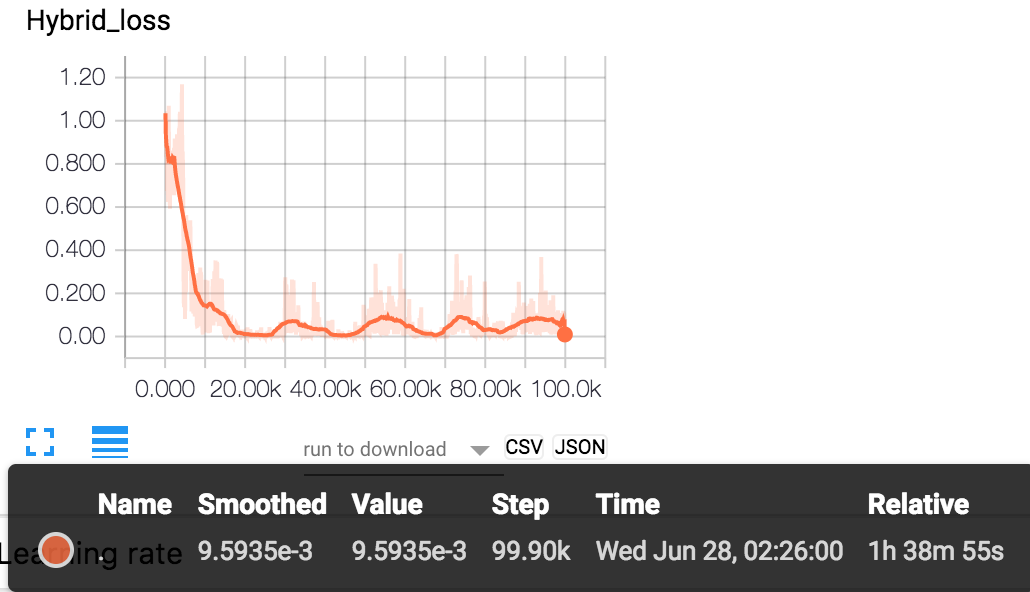
\includegraphics[width=0.75\linewidth]{config3/hybrid_loss}
  \caption{Configuration 3}
  \label{fig:sub2}
\end{subfigure}
\caption{Hybrid loss}
\label{fig:hybrid_loss}
\end{figure}


\begin{figure}
\centering
\begin{subfigure}{\textwidth}
  \centering
  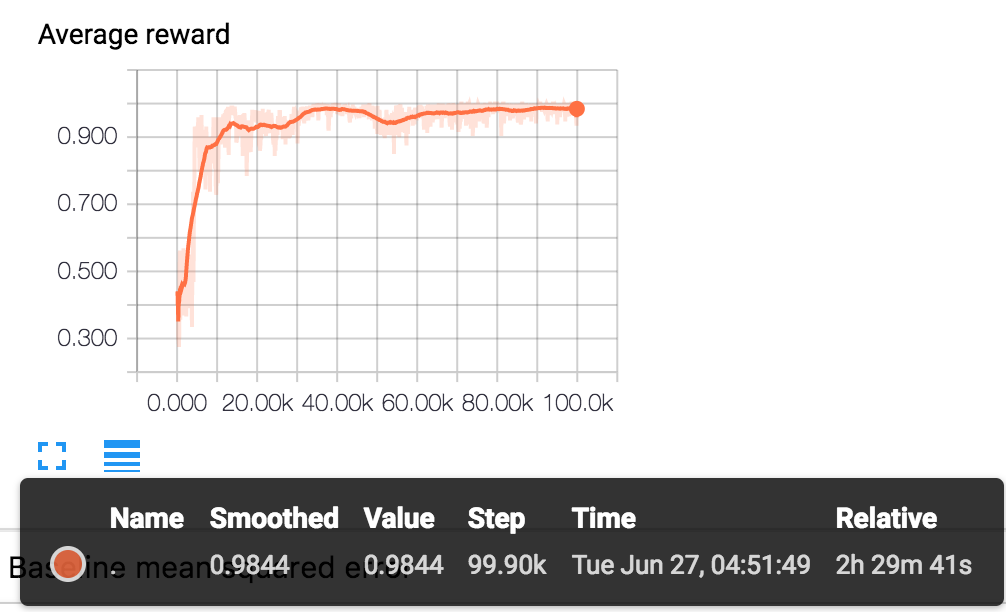
\includegraphics[width=0.75\linewidth]{config1/average_reward}
  \caption{Configuration 1}
  \label{fig:sub1}
\end{subfigure}
\begin{subfigure}{\textwidth}
  \centering
  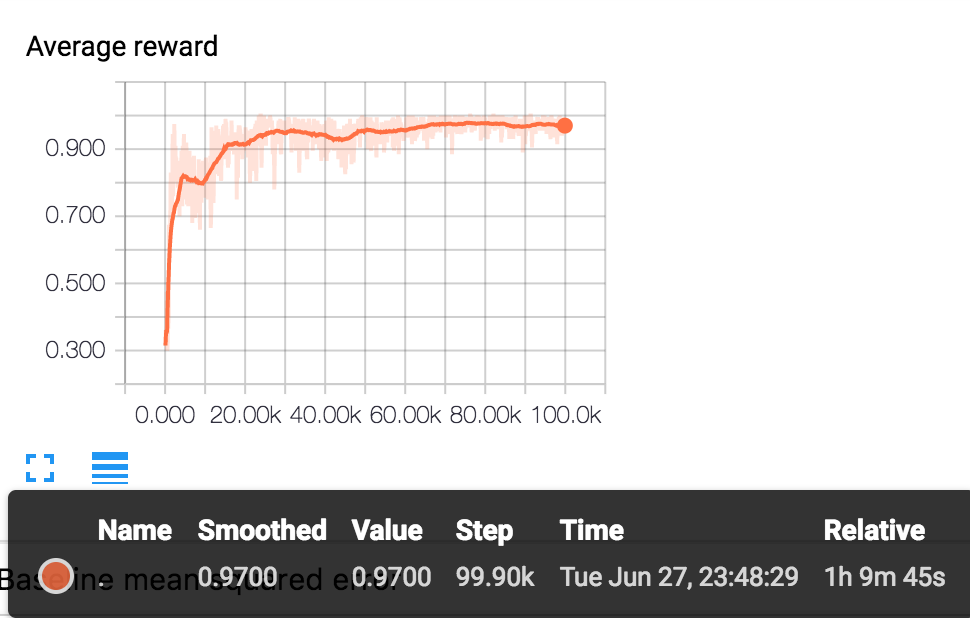
\includegraphics[width=0.75\linewidth]{config2/average_reward}
  \caption{Configuration 2}
  \label{fig:sub2}
\end{subfigure}
\begin{subfigure}{\textwidth}
  \centering
  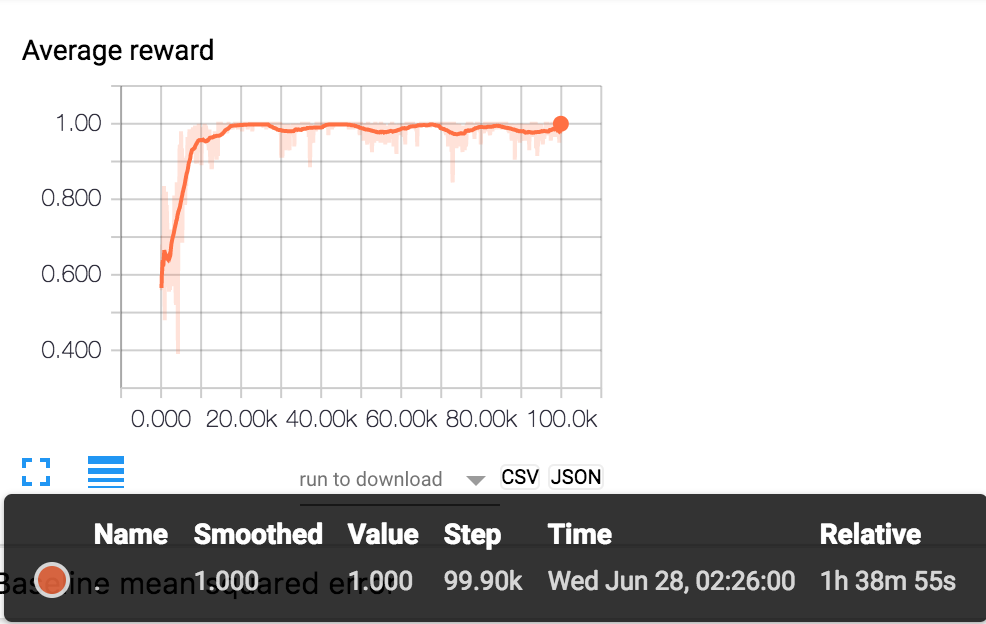
\includegraphics[width=0.75\linewidth]{config3/average_reward}
  \caption{Configuration 3}
  \label{fig:sub2}
\end{subfigure}
\caption{Average Reward}
\label{fig:average_reward}
\end{figure}


Broadly speaking, we found that it's required to
continue tuning the parameters of the model, as the figures clearly
highlighting the model's instability.

    \input{./tex/results}
	% Bibliography:
	\clearpage
	% \input{./tex/mybibliography.tex}
	\bibliographystyle{ieeetr}
	\bibliography{bibliography}
     \newpage
\pagenumbering{gobble}
\begin{center}
   \Large\textbf{Declaration of Authorship}
\end{center}

% \large
I hereby declare that the thesis submitted is my own unaided work. All direct or indirect
sources used are acknowledged as references.
I am aware that the thesis in digital form can be examined for the use of unauthorized
aid and in order to determine whether the thesis as a whole or parts incorporated
in it may be deemed as plagiarism. For the comparison of my work with existing
sources I agree that it shall be entered in a database where it shall also remain
after examination, to enable comparison with future theses submitted. Further rights
of reproduction and usage, however, are not granted here.
This paper was not previously presented to another examination board and has not
been published.
\vfill

\begin{center}
   \Large\textbf{Eigenständigkeitserklärung}
\end{center}

Hiermit versichere ich, dass ich die vorliegende Bachelorarbeit selbstständig und nur unter
Verwendung der angegebenen Quellen und Hilfsmittel verfasst habe. Die Arbeit wurde bisher
in gleicher oder ähnlicher Form keiner anderen Prüfungsbehörde vorgelegt.
\vfill

\noindent\begin{tabular}{ll}
\makebox[2.5in]{\hrulefill} & \makebox[2.5in]{\hrulefill}\\
first and last name & city, date, signature\\[8ex]% adds space between the two sets of signatures
\end{tabular}

\end{document}






% \begin{document}
% Here is some text, where we use \gls{apc}.
